\documentclass[11pt,a4paper]{article}

% ---- Packages ----
\usepackage[margin=1in]{geometry}
\usepackage{amsmath,amssymb,amsfonts}
\usepackage{booktabs}
\usepackage{graphicx}
\usepackage{enumitem}
\usepackage{hyperref}
\usepackage{multirow}
\usepackage{array}
\usepackage{caption}
\usepackage{xcolor}
\usepackage{float}
\usepackage[T1]{fontenc}
\usepackage{lmodern}

\graphicspath{{./}}
\DeclareGraphicsExtensions{.pdf,.png,.jpg}

\hypersetup{
    colorlinks=true,
    linkcolor=blue!60!black,
    citecolor=blue!60!black,
    urlcolor=blue!60!black
}

\definecolor{headerblue}{RGB}{0,51,102}
\definecolor{lightrow}{RGB}{240,245,250}

% ---- Custom commands ----
\newcommand{\Elo}{Elo}

% ---- Title ----
\title{\LARGE\textbf{Predicting Football Match Outcomes:\\A Multi-Model Ensemble Approach for the 2026 FIFA World Cup}}

\author{
  \begin{tabular}{c}
    S. Nou$^{1}$ \qquad GLM 5.1$^{2}$\\[0.5em]
    \small $^{1}$Independent Researcher \qquad $^{2}$Zhipu AI
  \end{tabular}
}

\date{June 2026}

\begin{document}

\sloppy

\maketitle

% ---- Abstract ----
\begin{abstract}
We present a machine learning system for predicting match outcomes in the 2026 FIFA World Cup, which features an expanded 48-team format across 12 groups. The system integrates \Elo{} ratings (computed from 49,477 international matches since 1872), FIFA rankings, Transfermarkt squad valuations, head-to-head records, and exponential weighted moving average form statistics into 80 engineered features. A weighted voting ensemble comprising XGBoost, Random Forest, Logistic Regression, and a multi-layer perceptron achieves 61.5\% test accuracy (log loss = 0.835) on held-out data, outperforming each individual model. A novel draw-aware calibration scheme adjusts predicted probabilities to reflect the empirical 25\% group-stage draw rate. Live validation on 13 completed World Cup matches yields 46.2\% accuracy (log loss = 1.05), with all five actual draws missed by argmax prediction despite well-calibrated draw probabilities. Monte Carlo simulation over 1,000 tournament runs identifies Mexico (7.9\%), Switzerland (5.6\%), and the United States (5.1\%) as the top contenders. We analyze the persistent difficulty of draw prediction in football and quantify the impact of host-nation advantage, confederation strength, and squad quality on tournament outcomes.
\end{abstract}

% ================================================================
\section{Introduction}
\label{sec:intro}

The FIFA World Cup is the most widely viewed sporting event in the world, and predicting its outcomes has attracted significant attention from both the statistical modeling and machine learning communities. The 2026 edition introduces a radical format change: 48 teams organized into 12 groups of four, with the top two from each group and the eight best third-placed teams advancing to a 32-team knockout bracket. This expansion creates new challenges for prediction models, as more teams from traditionally weaker confederations participate, and the group-stage dynamics change with the introduction of third-place qualifying spots.

Prior work on football prediction has explored \Elo{} rating systems~\cite{elo1978}, Poisson regression models for goal scoring~\cite{dixon1997}, and more recently, gradient-boosted decision trees~\cite{berrar2019}. The three-outcome nature of football matches (home win, draw, away win) poses a particular challenge, as draws occur in approximately 25\% of World Cup group-stage matches but are consistently underpredicted by classifiers trained to maximize accuracy.

In this paper, we present an end-to-end pipeline that: (1) computes \Elo{} ratings from historical match data spanning 1872--2025; (2) engineers 80 features incorporating form, head-to-head records, squad valuations, and confederation effects; (3) trains and evaluates a stacking ensemble of four heterogeneous classifiers; (4) applies draw-aware calibration for group-stage matches; and (5) simulates 1,000 tournament realizations to estimate advancement and winning probabilities for all 48 participating teams.

% ================================================================
\section{Data and Feature Engineering}
\label{sec:data}

\subsection{Data Sources}
\label{sec:data:sources}

The model integrates data from five primary sources: (1) International football results from 1872 to 2025, comprising 49,477 matches sourced via the Kaggle API~\cite{martj42}; (2) Historical FIFA Men's World Rankings with 67,492 entries and current rankings for 20 teams; (3) Transfermarkt squad market valuations for all 48 qualified teams, ranging from EUR\,20M (Qatar) to EUR\,1.52B (France); (4) Wikipedia-sourced historical World Cup results (117 entries) and 2026 group stage fixtures; and (5) Live 2026 World Cup results from Wikipedia, currently covering 13 completed matches.

Team name normalization is performed via a 23-entry mapping dictionary to reconcile naming conventions across sources (e.g., USA$\to$United States, Korea Republic$\to$South Korea). Confederation membership for 104 countries is maintained in a mapping table, enabling same-confederation features and confederation-average fallbacks for missing squad data. The final match feature dataset contains 49,413 rows after filtering and cleaning.

\subsection{\Elo{} Rating System}
\label{sec:elo}

We compute \Elo{} ratings using a tournament-adaptive K-factor system. The expected score for the home team is computed as:
\begin{equation}
\label{eq:elo_expected}
E_H = \frac{1}{1 + 10^{(R_A - R_H^*) / 400}}
\end{equation}
where $R_H^* = R_H + \delta_H$, and $\delta_H = 100$ (\texttt{ELO\_HOME\_ADVANTAGE}) for home matches and 0 for neutral-venue matches. Ratings are updated after each match as:
\begin{equation}
\label{eq:elo_update}
R_H' = R_H + K_T \cdot (S_H - E_H)
\end{equation}
where $S_H$ is 1.0 for a home win, 0.5 for a draw, and 0.0 for an away win. K-factors are tournament-specific: 80 for World Cup matches, 60 for qualifiers, 40 for friendlies, and 50 as the default. Initial ratings are set at 1000.

A three-class probability model extends the binary \Elo{} framework to handle draws. The draw probability is computed as:
\begin{equation}
\label{eq:draw_prob}
P_D = \min\!\Big(\varphi \cdot (1 - |E_H - E_A|),\; \min\!\big(\max(0.05,\, \min(E_H, E_A)),\; 0.35\big)\Big)
\end{equation}
with $\varphi = 0.30$ (\texttt{ELO\_DRAW\_FACTOR}). This formulation ensures draws are most likely when teams are evenly matched ($E_H \approx E_A$), bounded between 5\% and 35\%, and never exceed the weaker team's expected score. The remaining probability is distributed proportionally:
\begin{equation}
\label{eq:prob_dist}
P_H = (1 - P_D) \cdot \frac{E_H}{E_H + E_A}, \qquad P_A = (1 - P_D) \cdot \frac{E_A}{E_H + E_A}
\end{equation}

\begin{figure}[t]
\centering
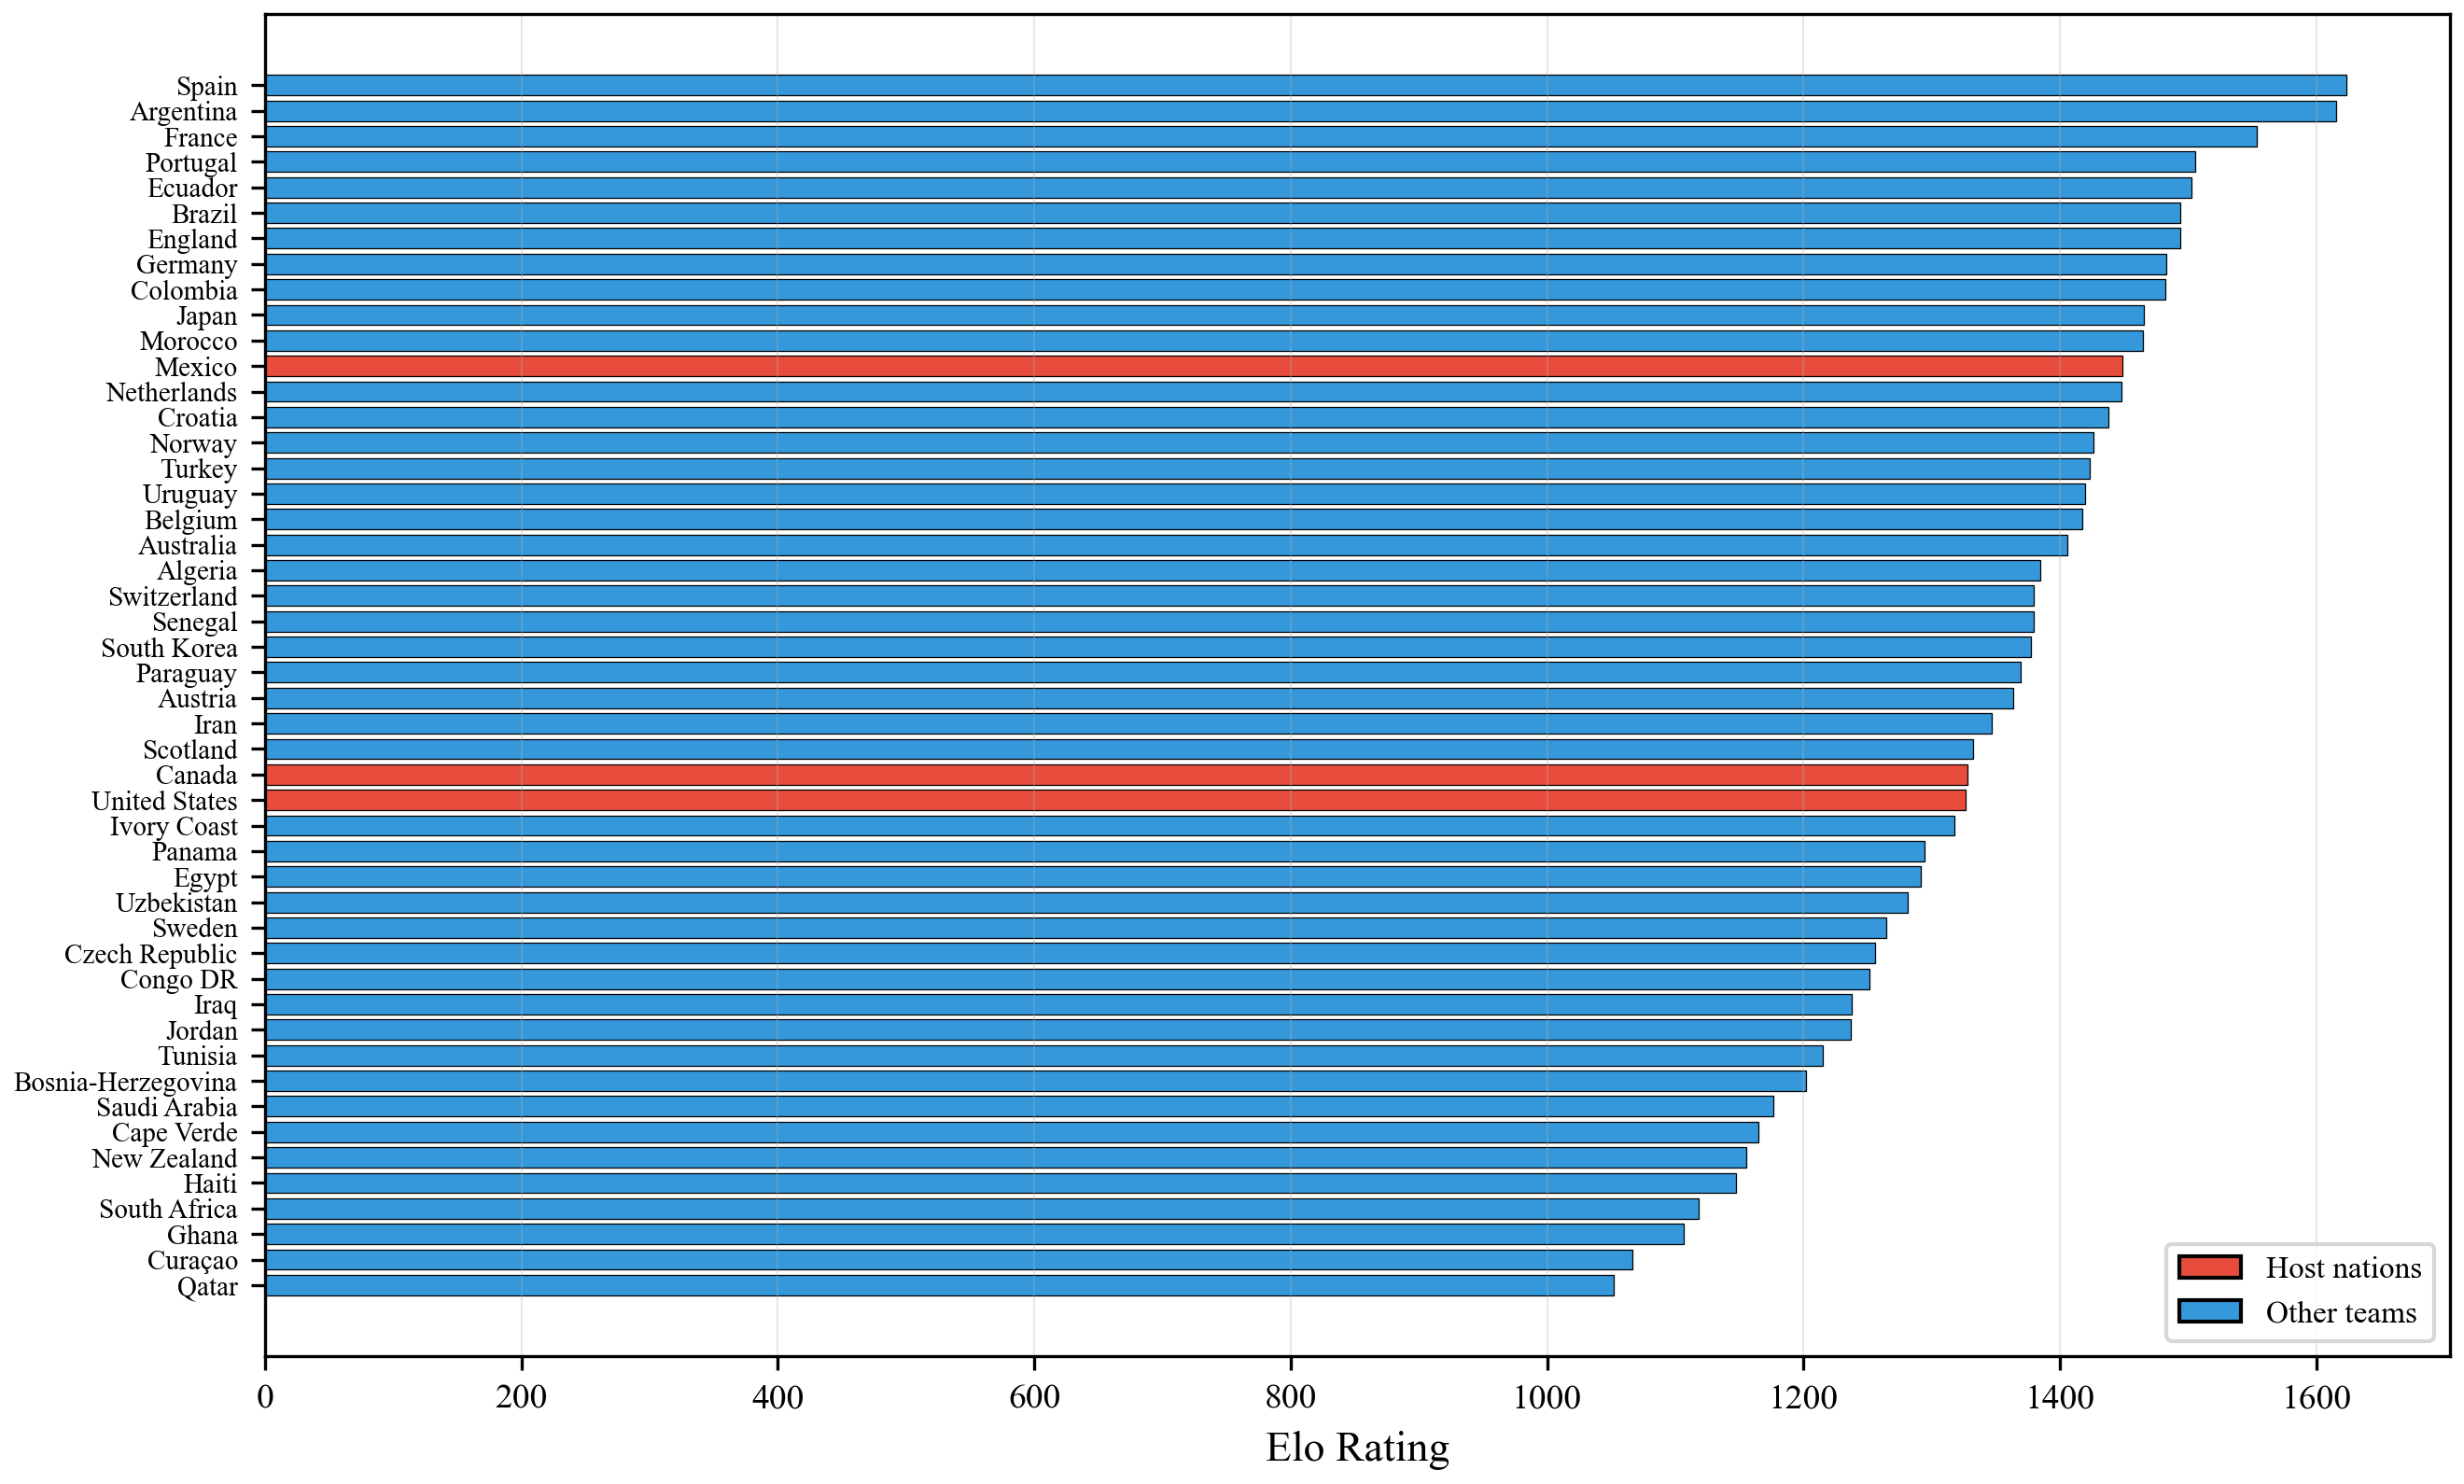
\includegraphics[width=\textwidth]{fig_elo_ratings.png}
\caption{Elo ratings of the 48 qualified teams for the 2026 FIFA World Cup, computed from 49,477 historical international matches. Host nations (Mexico, United States, Canada) are highlighted in red.}
\label{fig:elo_ratings}
\end{figure}

\subsection{Feature Engineering}
\label{sec:features}

We engineer 80 features organized into 10 categories (Table~\ref{tab:features}). Core features (27) include \Elo{} ratings, FIFA rankings and points, home advantage indicators, confederation match flags, and \Elo{}-derived draw probabilities. Form features (28) capture recent team performance over the last 5 and 10 matches, including win/draw/loss rates, goal averages, and clean sheet rates for both home and away contexts. Exponentially weighted moving average (EWMA) form features (6) with $\lambda = 0.3$ give greater weight to recent results:
\begin{equation}
\label{eq:ewma}
\bar{x}_{\text{EWM}} = \frac{\sum_{i=1}^{n} w_i \, x_i}{\sum_{i=1}^{n} w_i}, \qquad w_i = e^{-\lambda \cdot i}
\end{equation}
Head-to-head features (6) summarize the last 5 meetings between each pair. Squad quality features (8) from Transfermarkt include total squad market value, average player value, and top player value for each team. Odds features (3) from the-odds-api provide implied probabilities for each outcome.

\begin{table}[t]
\centering
\caption{Feature categories and counts. The full feature set comprises 80 features, with 27 core features always present and 53 optional features subject to data availability.}
\label{tab:features}
\begin{tabular}{lc p{8.5cm}}
\toprule
\textbf{Category} & \textbf{N} & \textbf{Description} \\
\midrule
\Elo{}         & 7 & Ratings, delta, win/draw/away probabilities \\
FIFA Rankings  & 6 & Rank, points, delta, absolute delta \\
Match Context  & 5 & Neutral, home advantage, host nation, WC/knockout flags \\
Draw Features  & 3 & Combined prob, elo\_close, draw\_tendency \\
Form (H/A)     & 28 & Last 5/10 match stats, EWM rates, goals, clean sheets \\
Head-to-Head   & 6 & Last 5 meetings: wins, draws, goals \\
Squad Quality  & 8 & Transfermarkt market values, player values \\
SoS            & 2 & Average opponent \Elo{} rating \\
Tourn.\ Draw Rate & 1 & Historical draw rate by tournament type \\
Odds           & 3 & Implied probabilities from betting markets \\
Interactions   & 2 & \Elo{} $\times$ home\_advantage, rank $\times$ confederation \\
\midrule
\textbf{Total} & \textbf{80} & \\
\bottomrule
\end{tabular}
\end{table}

\begin{figure}[t]
\centering
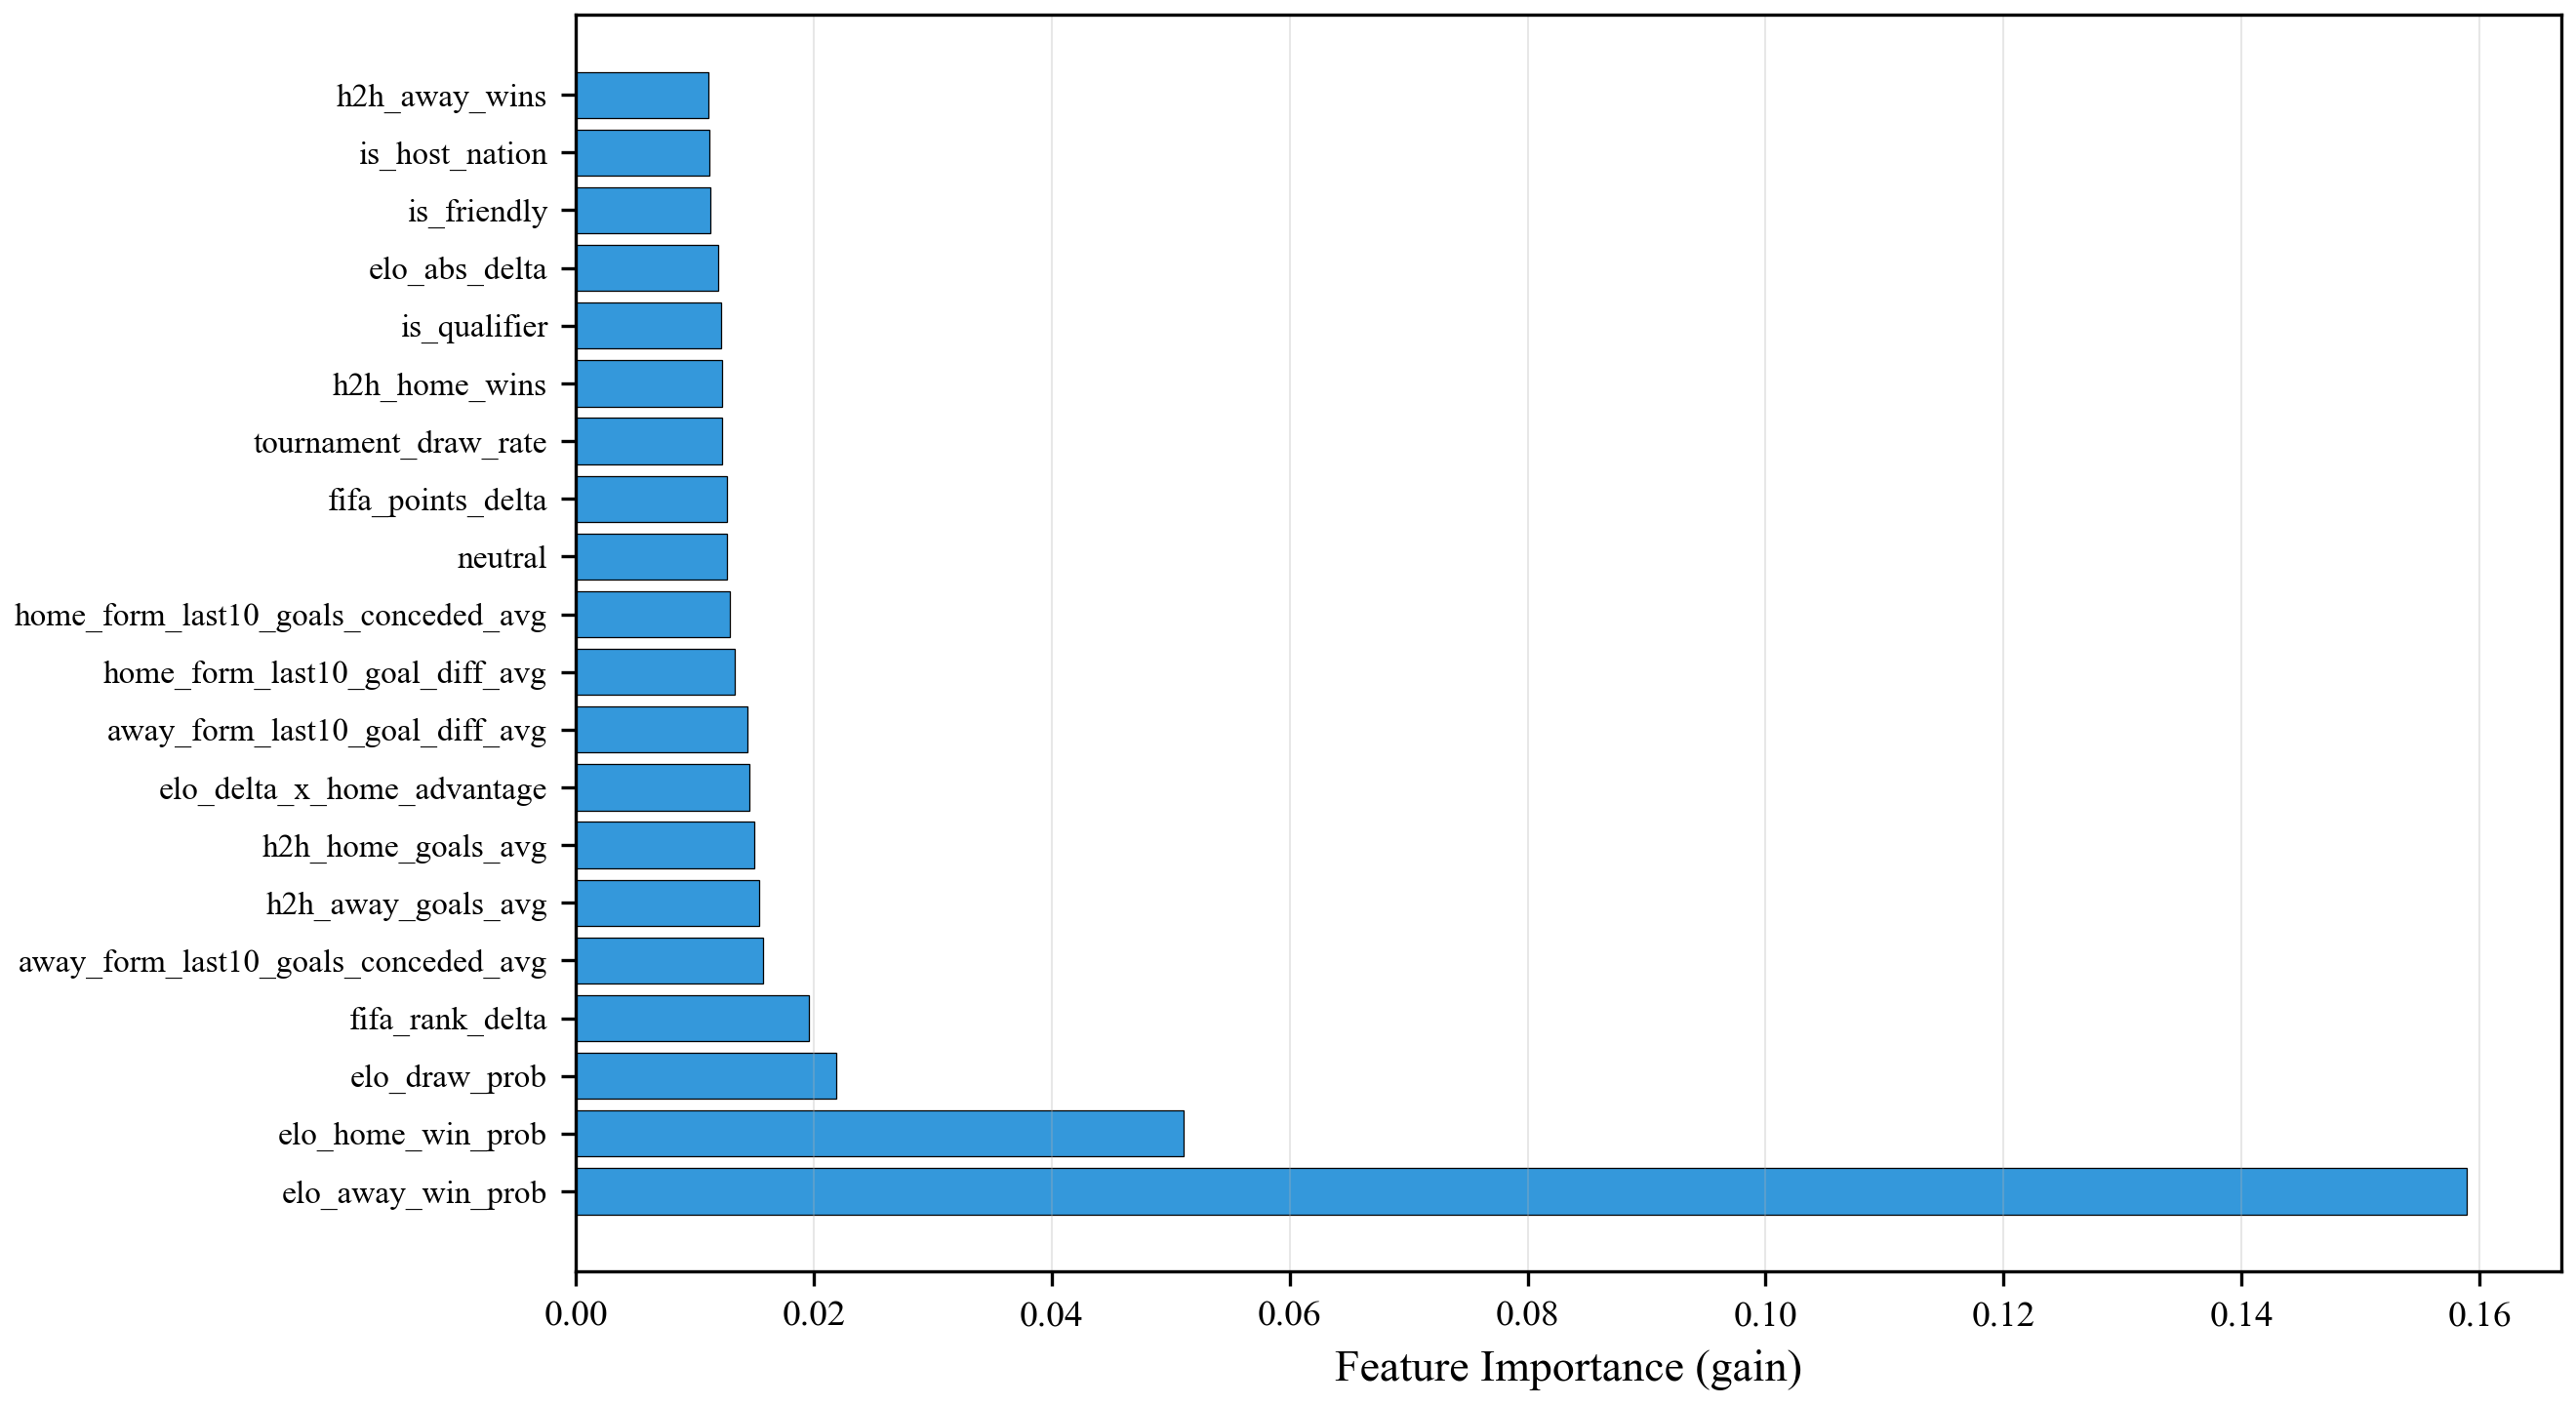
\includegraphics[width=\textwidth]{fig_feature_importance.png}
\caption{Top 20 feature importances from the XGBoost model, ranked by gain. Elo-derived features dominate the top positions, confirming the importance of rating-based signals.}
\label{fig:feature_importance}
\end{figure}

% ================================================================
\section{Model Architecture}
\label{sec:model}

\subsection{Individual Models}
\label{sec:model:individual}

We train four heterogeneous classifiers, each selected for complementary strengths in the ensemble:

\begin{itemize}[leftmargin=1.5em]
\item \textbf{XGBoost}: Optuna-optimized with 20 trials of Bayesian optimization using 3-fold time-series cross-validation. Search space includes $n_\text{estimators} \in [100, 500]$, $\text{max\_depth} \in [3, 10]$, $\text{learning\_rate} \in [0.01, 0.3]$ (log-uniform), and regularization parameters. Draw class weight is $4\times$. Test accuracy: 50.5\%, log loss: 0.955.

\item \textbf{Random Forest}: Grid search over $n_\text{estimators} \in \{100, 200\}$, $\text{max\_depth} \in \{10, 20\}$, $\text{min\_samples\_split} \in \{2, 5\}$, with \texttt{class\_weight='balanced'}. Test accuracy: 59.3\%, log loss: 0.857.

\item \textbf{Logistic Regression}: L2-regularized with StandardScaler preprocessing. Grid search over $C \in \{0.01, 0.1, 1.0, 10.0\}$ with \texttt{class\_weight='balanced'}. Test accuracy: 57.9\%, log loss: 0.874.

\item \textbf{Neural Network (MLP)}: Three hidden layers (128, 64, 32) with ReLU activation, Adam optimizer, adaptive learning rate (init: $10^{-3}$), $\alpha = 10^{-3}$ (L2), batch size 256, early stopping with patience 10. Draw class weight is $8\times$. Test accuracy: 35.9\%, log loss: 1.732. Retained for ensemble diversity despite worst individual performance.
\end{itemize}

\subsection{Ensemble Selection}
\label{sec:model:ensemble}

The final model is selected by minimum validation log loss from three candidate ensembles: (1) a uniform soft-voting ensemble (\texttt{VotingEnsemble}), (2) a weighted soft-voting ensemble (\texttt{WeightedVotingEnsemble}) using inverse-log-loss weights, and (3) a stacking ensemble (\texttt{StackingClassifier}) with a Logistic Regression meta-learner. The current best model is the \texttt{WeightedVotingEnsemble} with weights proportional to the inverse of each base model's validation log loss: $w_i = (1/\text{LL}_i) / \sum_j (1/\text{LL}_j)$, yielding weights of approximately 0.29 for Random Forest, 0.29 for Logistic Regression, 0.26 for XGBoost, and 0.15 for Neural Network. Crucially, the meta-learner and voting weights do \textbf{not} use \texttt{class\_weight='balanced'}---empirically, balanced weights on the StackingClassifier meta-learner caused massive draw overprediction (353 draws predicted vs.\ 220 expected), while removing it yielded both better log loss and calibration.

The ensemble achieves test accuracy of 61.5\% with log loss 0.835, outperforming all individual models (Table~\ref{tab:model_perf}). Model selection is by minimum validation log loss; ties are broken by maximum accuracy.

\begin{table}[t]
\centering
\caption{Model performance on the test set (matches after 2023, $n = 2{,}552$). Brier scores are per-class. H = home win, D = draw, A = away win.}
\label{tab:model_perf}
\begin{tabular}{lcccccc}
\toprule
\textbf{Model} & \textbf{Acc.} & \textbf{LL} & \textbf{Br(H)} & \textbf{Br(D)} & \textbf{Br(A)} & \textbf{Avg} \\
\midrule
WeightedVoting Ensemble & 0.615 & 0.835 & 0.174 & 0.172 & 0.144 & 0.163 \\
Random Forest        & 0.593 & 0.857 & 0.181 & 0.177 & 0.147 & 0.168 \\
Logistic Regression  & 0.579 & 0.874 & 0.189 & 0.181 & 0.146 & 0.172 \\
XGBoost              & 0.505 & 0.955 & 0.194 & 0.227 & 0.160 & 0.194 \\
Neural Network       & 0.359 & 1.732 & 0.304 & 0.427 & 0.222 & 0.318 \\
\bottomrule
\end{tabular}
\end{table}

\begin{figure}[t]
\centering
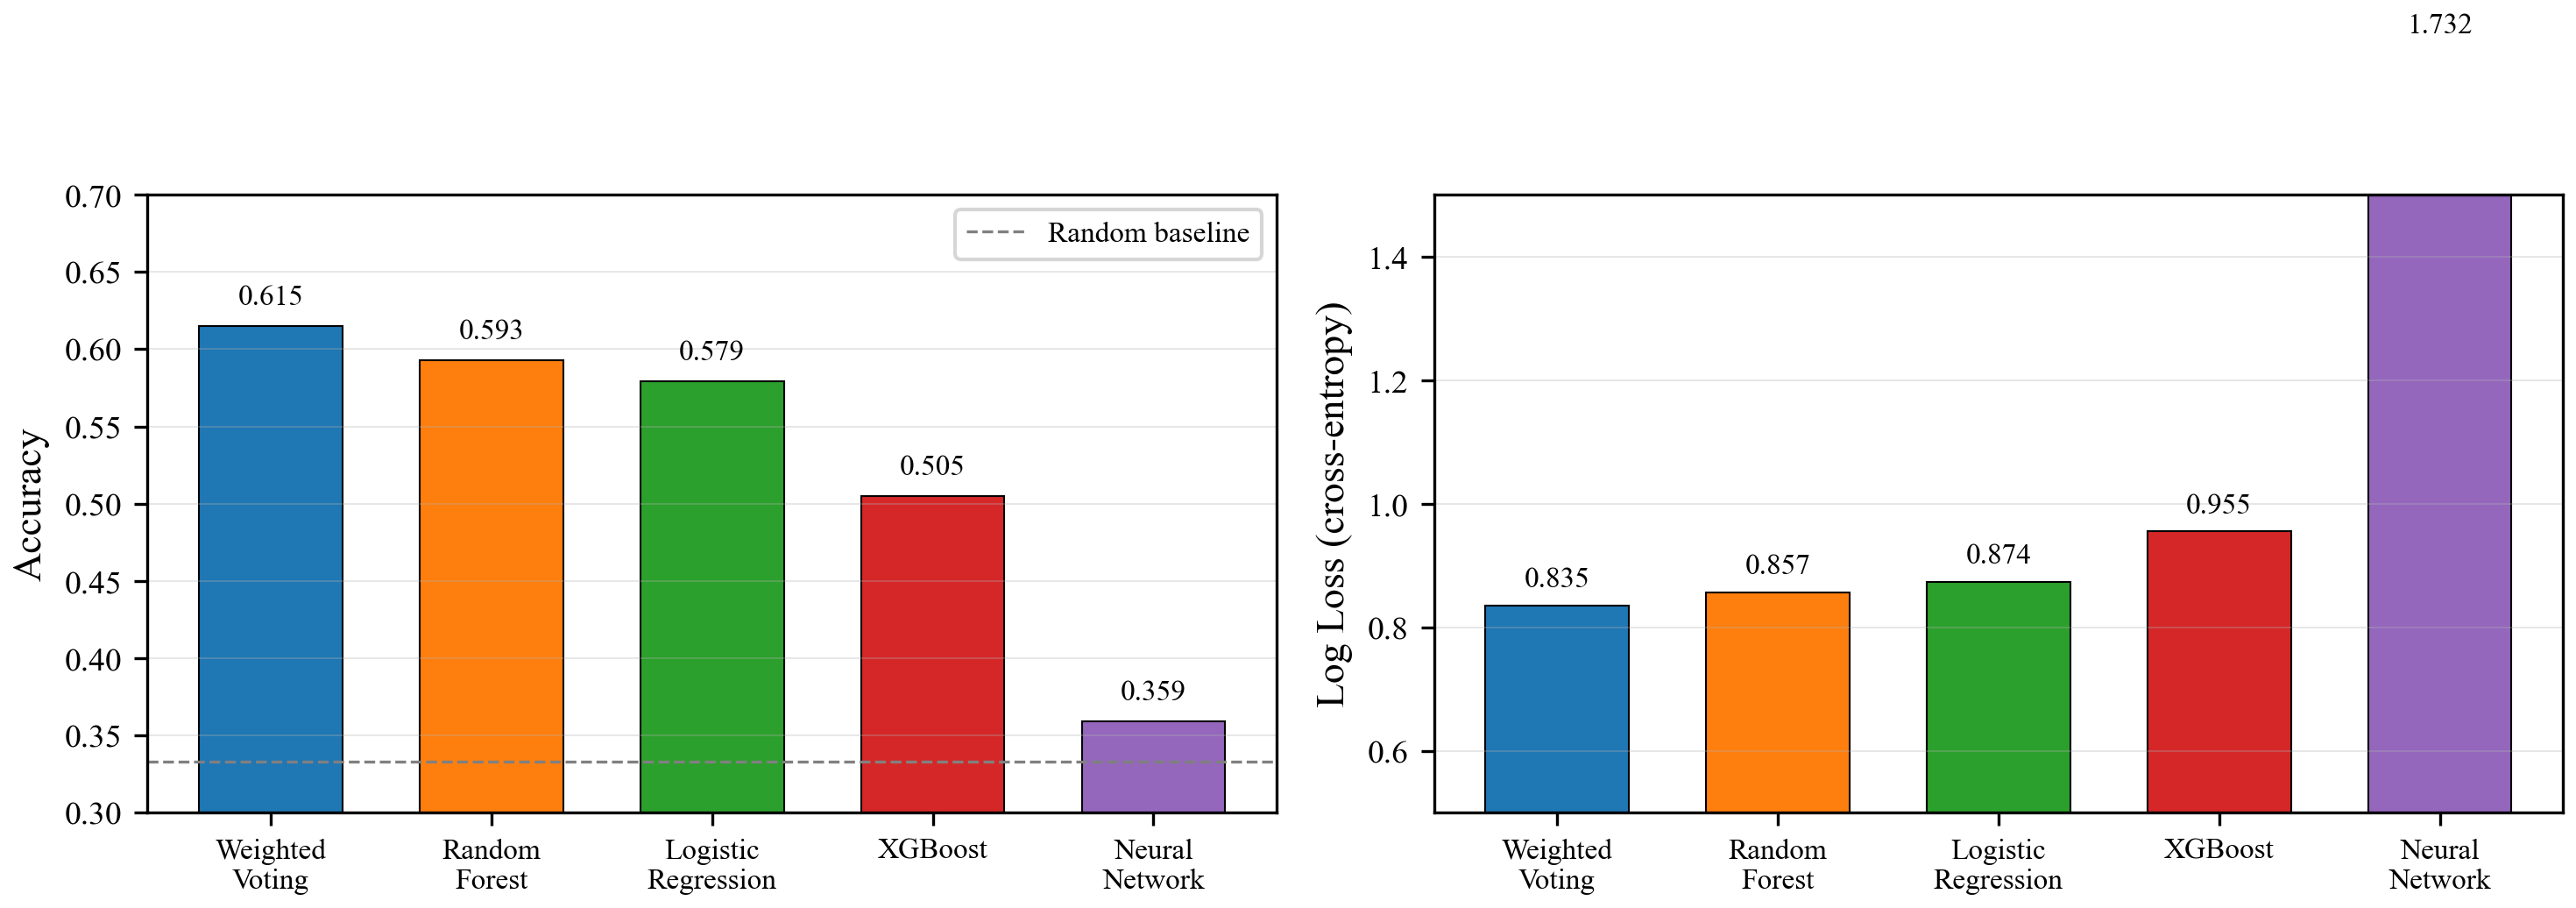
\includegraphics[width=\textwidth]{fig_model_comparison.png}
\caption{Model comparison on the test set ($n = 2{,}552$ matches after 2023). Left: classification accuracy with random baseline (dashed line at 0.333). Right: log loss (cross-entropy), where lower is better. The WeightedVoting Ensemble achieves the best performance on both metrics.}
\label{fig:model_comparison}
\end{figure}

\begin{figure}[t]
\centering
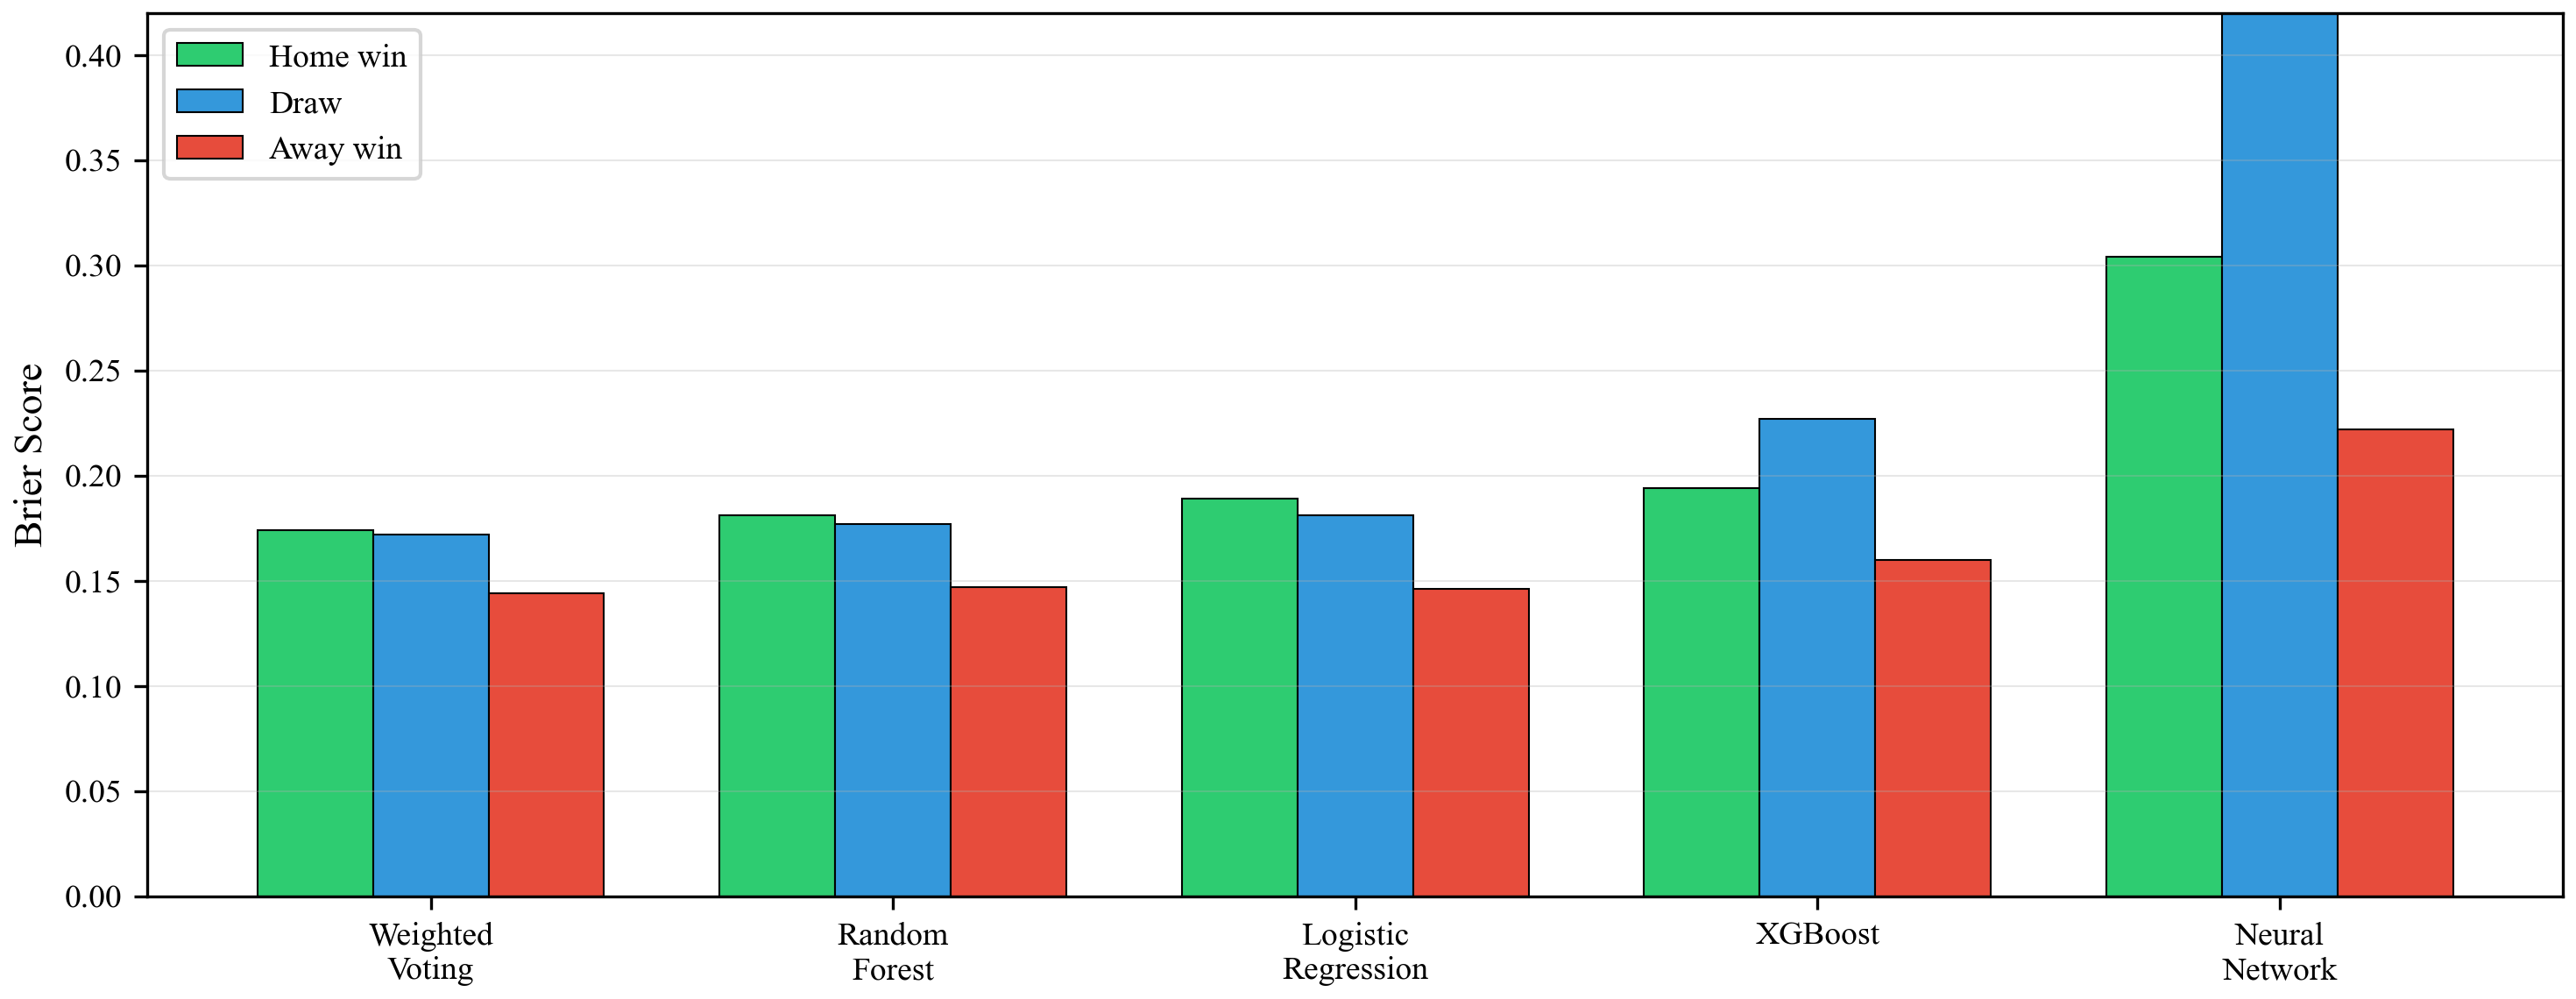
\includegraphics[width=\textwidth]{fig_brier_scores.png}
\caption{Per-class Brier scores by model. The draw class (blue) consistently has the highest Brier score across all models, reflecting the difficulty of draw prediction. The WeightedVoting Ensemble achieves the most balanced performance across classes.}
\label{fig:brier_scores}
\end{figure}

\subsection{Draw Handling}
\label{sec:model:draw}

Draw prediction is the central challenge of three-outcome football modeling. We employ multiple strategies to address the systematic underprediction of draws:

\begin{itemize}[leftmargin=1.5em]
\item \textbf{Sample weighting}: Draw samples receive $4\times$ weight in XGBoost and $8\times$ in the Neural Network; Random Forest and Logistic Regression use \texttt{class\_weight='balanced'} for automatic class rebalancing.

\item \textbf{Feature engineering}: Draw-predictive features include \texttt{elo\_close} ($|\Delta_{\text{elo}}| < 100$), \texttt{fifa\_close} ($|\Delta_{\text{rank}}| < 20$), \texttt{combined\_draw\_prob}, and \texttt{draw\_tendency}.

\item \textbf{Draw calibration}: In group-stage simulation, probabilities are post-hoc adjusted so that $P(\text{draw}) \geq 25\%$ (the empirical WC group draw rate). If below 25\%, the deficit is redistributed proportionally from win probabilities.

\item \textbf{Knockout draw redistribution}: In knockout matches, 70\% of the draw probability is redistributed to home (55\%) and away (45\%) win probabilities:
\begin{equation}
\label{eq:knockout_redist}
\hat{P}_H = P_H + 0.7 \cdot P_D \cdot 0.55, \qquad \hat{P}_A = P_A + 0.7 \cdot P_D \cdot 0.45
\end{equation}
\end{itemize}

Despite these measures, argmax prediction still fails to classify any match as a draw in live validation. The draw probability is well-calibrated (mean predicted draw probability for actual draws is 0.21), but the model rarely assigns draw as the highest probability. This reflects a fundamental tension: draws are inherently uncertain events where the evidence for a draw is often weaker than for either team winning, even when the true outcome is a draw.

% ================================================================
\section{Tournament Simulation}
\label{sec:simulation}

We simulate the 2026 FIFA World Cup using Monte Carlo methods over 1,000 independent tournament realizations. The simulation proceeds through three phases:

\textbf{Group stage}: For each of the 12 groups, all 6 round-robin matches are simulated using the ensemble's predicted probabilities, with draw calibration applied to ensure at least 25\% draw probability per match. Points (3/1/0), goal difference, and goals scored are tracked to determine group standings. The top two teams from each group and the eight best third-placed teams advance.

\textbf{Knockout stage}: The Round of 32 bracket is constructed according to a fixed mapping (Group A winner vs Group B runner-up, etc.), and each knockout match is simulated as a binary outcome by redistributing 70\% of the draw probability (Equation~\ref{eq:knockout_redist}). Goal generation uses a Poisson model with $\lambda = 1.5$ for home winners and $\lambda = 1.3$ for away winners.

\textbf{Live results integration}: For the 13 completed World Cup matches, actual results replace simulated outcomes, ensuring group standings reflect the current tournament state.

\subsection{Simulation Results}
\label{sec:simulation:results}

Table~\ref{tab:simulation} presents the top 15 teams by estimated winning probability. The three host nations (Mexico, United States, Canada) collectively hold a 17.3\% probability of winning the tournament, with Mexico benefiting from both home advantage and a favorable group draw.

\begin{table}[t]
\centering
\caption{Top 15 teams by estimated probability of winning the 2026 FIFA World Cup, based on 1,000 Monte Carlo simulations. R32 probabilities can exceed 100\% due to third-place qualifying rules (8 of 12 third-placed teams advance).}
\label{tab:simulation}
\begin{tabular}{clcccccc}
\toprule
\textbf{Rank} & \textbf{Team} & \textbf{Win\%} & \textbf{R32\%} & \textbf{Ro16\%} & \textbf{QF\%} & \textbf{SF\%} & \textbf{Final\%} \\
\midrule
1  & Mexico         & 7.9  & 101.7 & 60.1 & 33.2 & 15.6 & 7.9  \\
2  & Switzerland    & 5.6  & 71.0  & 37.0 & 20.3 & 10.4 & 5.6  \\
3  & United States  & 5.1  & 92.6  & 43.5 & 19.7 & 10.9 & 5.1  \\
4  & Ivory Coast    & 4.8  & 61.7  & 31.2 & 18.0 & 6.8  & 4.8  \\
5  & France         & 4.6  & 49.9  & 32.2 & 17.7 & 10.7 & 4.6  \\
6  & Canada         & 4.3  & 68.5  & 34.4 & 18.8 & 9.3  & 4.3  \\
7  & Argentina      & 4.2  & 48.4  & 28.2 & 18.0 & 9.7  & 4.2  \\
8  & Spain          & 4.1  & 102.5 & 52.8 & 22.4 & 5.7  & 4.1  \\
9  & Brazil         & 4.0  & 70.2  & 39.5 & 17.3 & 8.7  & 4.0  \\
10 & Germany        & 3.8  & 95.3  & 56.0 & 33.9 & 7.7  & 3.8  \\
11 & Scotland       & 3.2  & 64.1  & 33.1 & 14.9 & 6.0  & 3.2  \\
12 & Morocco        & 3.2  & 55.6  & 28.3 & 12.6 & 6.4  & 3.2  \\
13 & South Korea    & 3.1  & 52.9  & 21.2 & 10.8 & 5.3  & 3.1  \\
14 & Netherlands    & 2.7  & 63.2  & 33.4 & 20.1 & 4.9  & 2.7  \\
15 & Belgium        & 2.7  & 84.6  & 51.2 & 22.6 & 4.8  & 2.7  \\
\bottomrule
\end{tabular}
\end{table}

\begin{figure}[t]
\centering
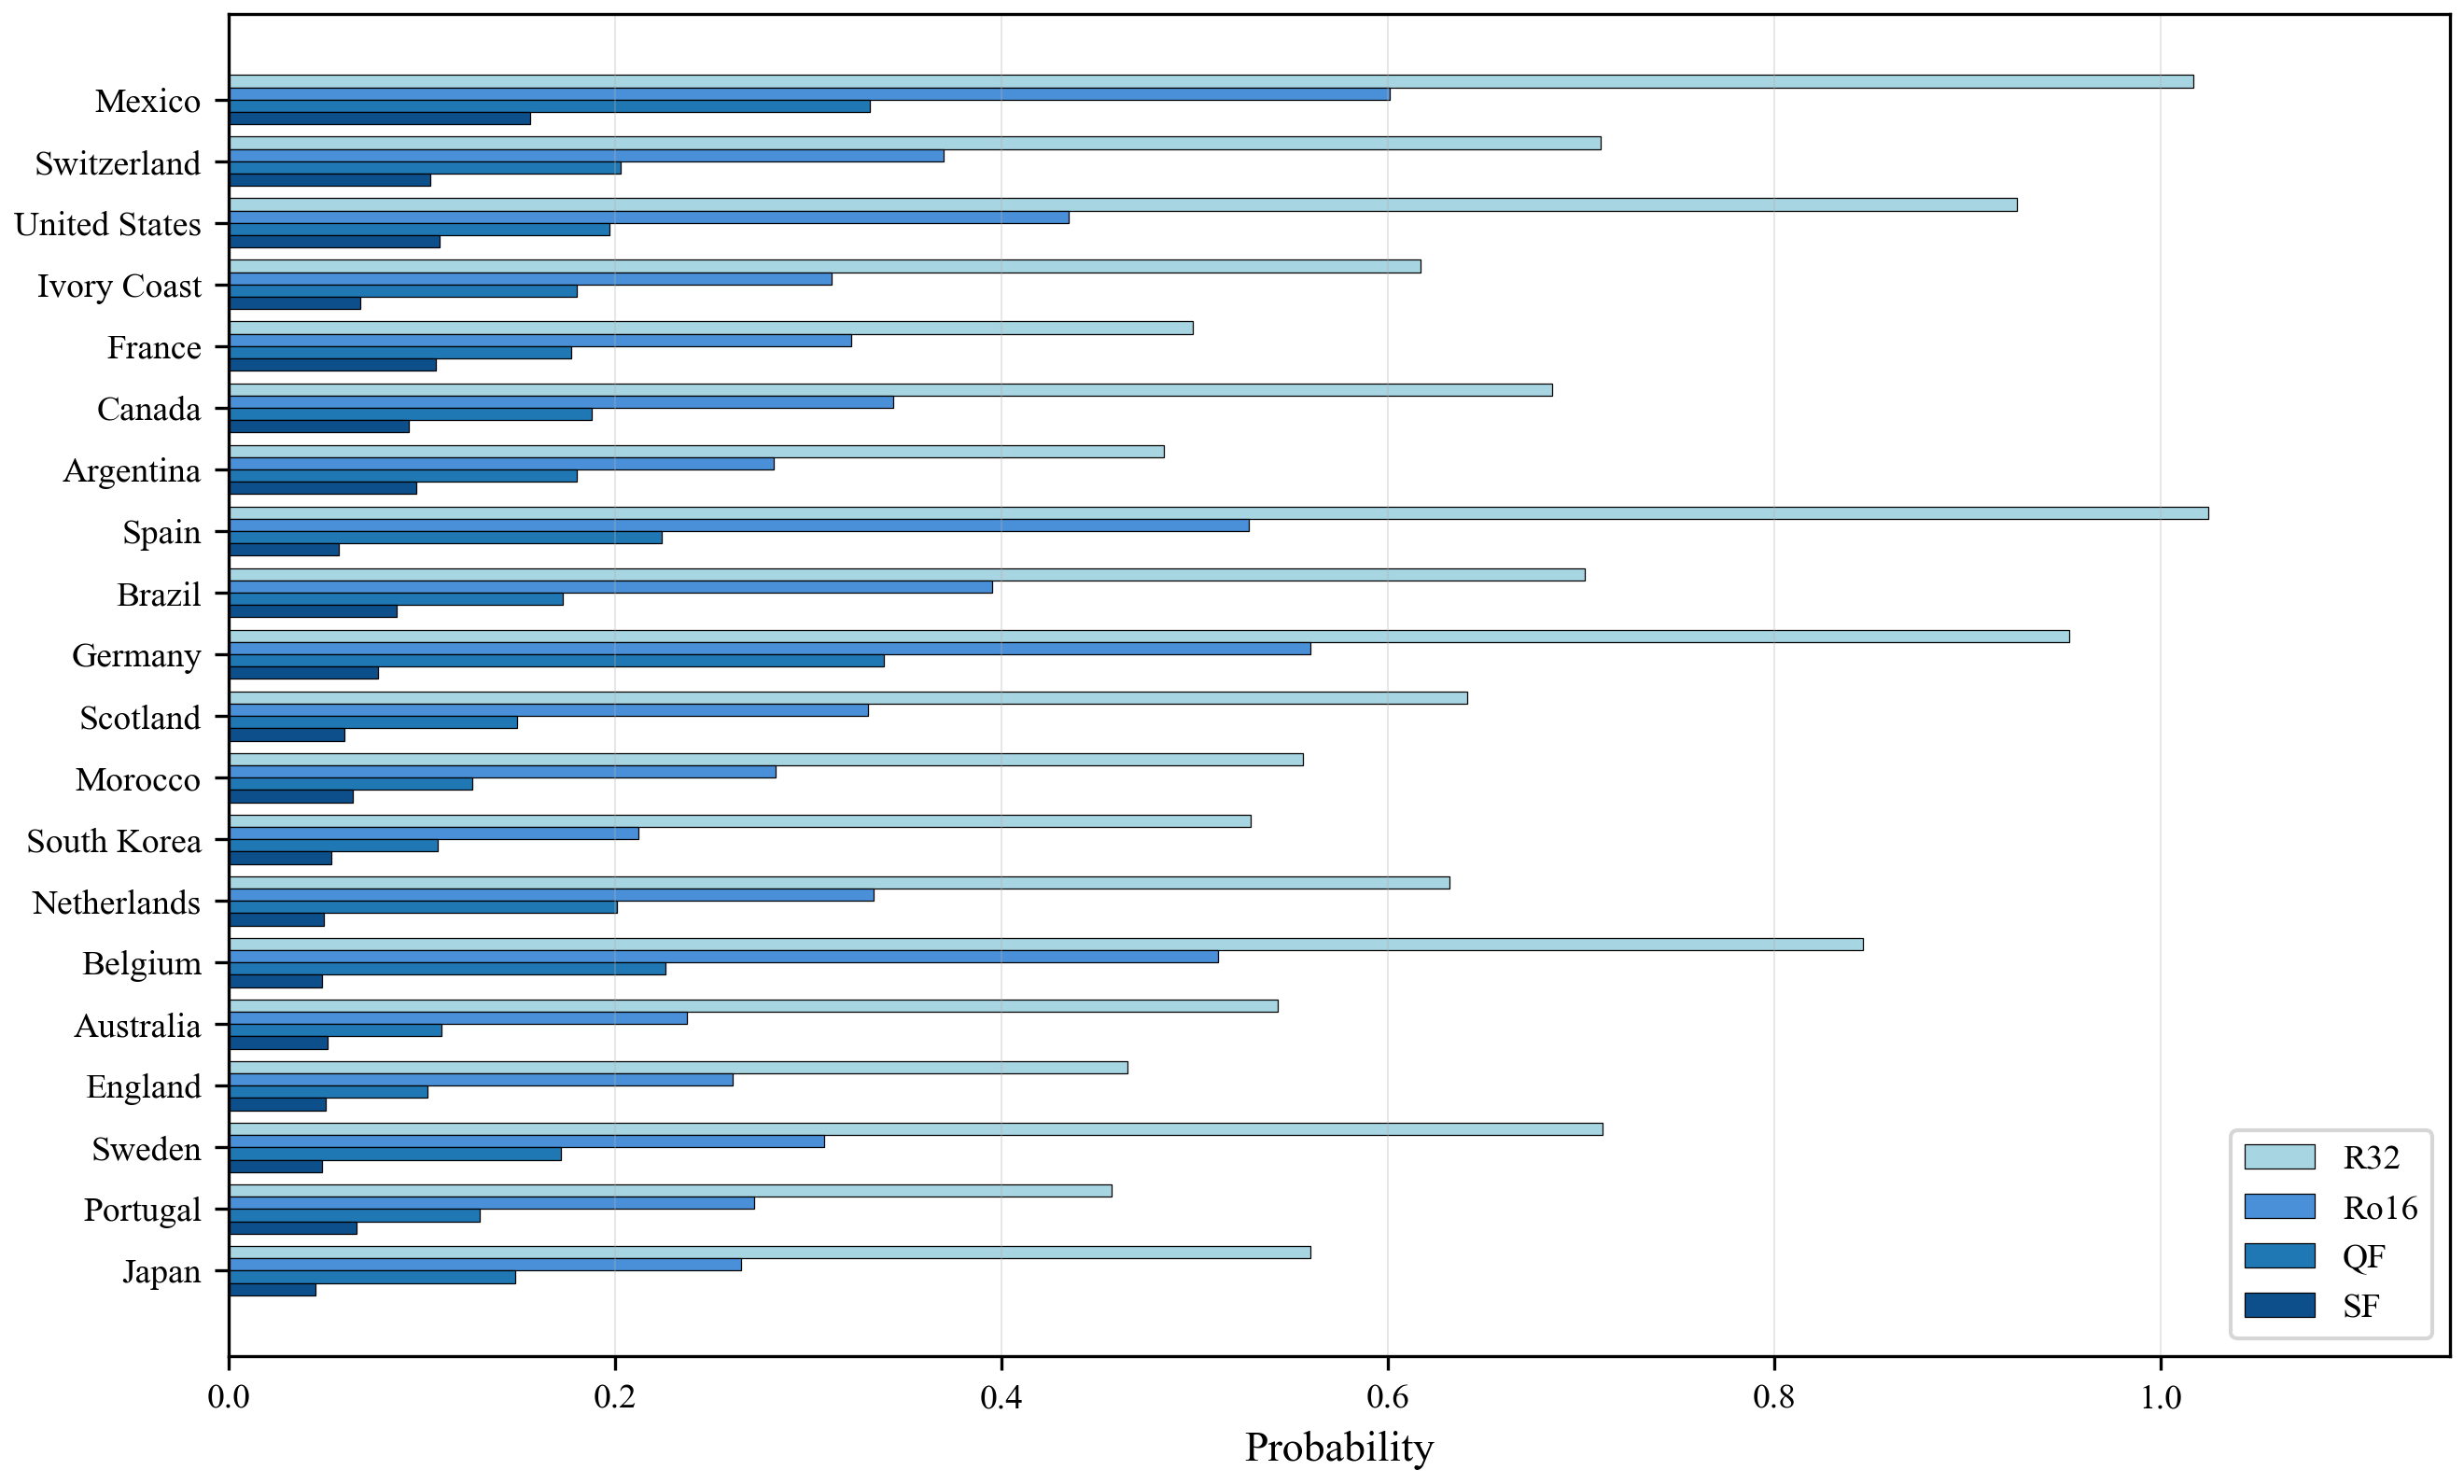
\includegraphics[width=\textwidth]{fig_tournament_probs.png}
\caption{Tournament advancement probabilities for the top 20 teams, based on 1,000 Monte Carlo simulations. R32 probabilities can exceed 100\% due to third-place qualifying rules. Host nations are highlighted.}
\label{fig:tournament_probs}
\end{figure}

% ================================================================
\section{Live Validation}
\label{sec:validation}

We validate the model against 13 completed matches from the 2026 World Cup group stage (as of June 15, 2026). Table~\ref{tab:live} shows per-match predictions.

\begin{table}[t]
\centering
\caption{Per-match predictions on 13 completed WC 2026 matches. $P(H)$, $P(D)$, $P(A)$ = predicted probabilities. D/Max = draw probability divided by $\max(P(H), P(A))$. All five actual draws are missed by argmax prediction.}
\label{tab:live}
\small
\begin{tabular}{llcccrccc}
\toprule
\textbf{Match} & \textbf{Score} & \textbf{Actual} & \textbf{Pred.} & $P(H)$ & $P(D)$ & $P(A)$ & \textbf{D/Max} & \\
\midrule
MEX vs RSA & 2--0 & Home & Home & 0.82 & 0.12 & 0.06 & 0.14 & \\
KOR vs CZE & 2--1 & Home & Home & 0.40 & 0.29 & 0.31 & 0.73 & \\
CAN vs BIH & 1--1 & Draw & Home & 0.69 & 0.20 & 0.11 & 0.29 & \\
USA vs PAR & 4--1 & Home & Home & 0.47 & 0.24 & 0.29 & 0.52 & \\
QAT vs SUI & 1--1 & Draw & Away & 0.10 & 0.16 & 0.75 & 0.21 & \\
BRA vs MAR & 1--1 & Draw & Home & 0.46 & 0.28 & 0.25 & 0.61 & \\
HAI vs SCO & 0--1 & Away & Away & 0.17 & 0.22 & 0.61 & 0.37 & \\
AUS vs TUR & 2--0 & Home & Away & 0.22 & 0.24 & 0.55 & 0.43 & \\
GER vs CUW & 7--1 & Home & Home & 0.78 & 0.14 & 0.08 & 0.17 & \\
NED vs JPN & 2--2 & Draw & Home & 0.45 & 0.29 & 0.26 & 0.64 & \\
CIV vs ECU & 1--0 & Home & Away & 0.30 & 0.28 & 0.42 & 0.66 & \\
SWE vs TUN & 5--1 & Home & Home & 0.54 & 0.22 & 0.25 & 0.41 & \\
ESP vs CPV & 0--0 & Draw & Home & 0.78 & 0.14 & 0.08 & 0.18 & \\
\bottomrule
\end{tabular}
\end{table}

\begin{figure}[t]
\centering
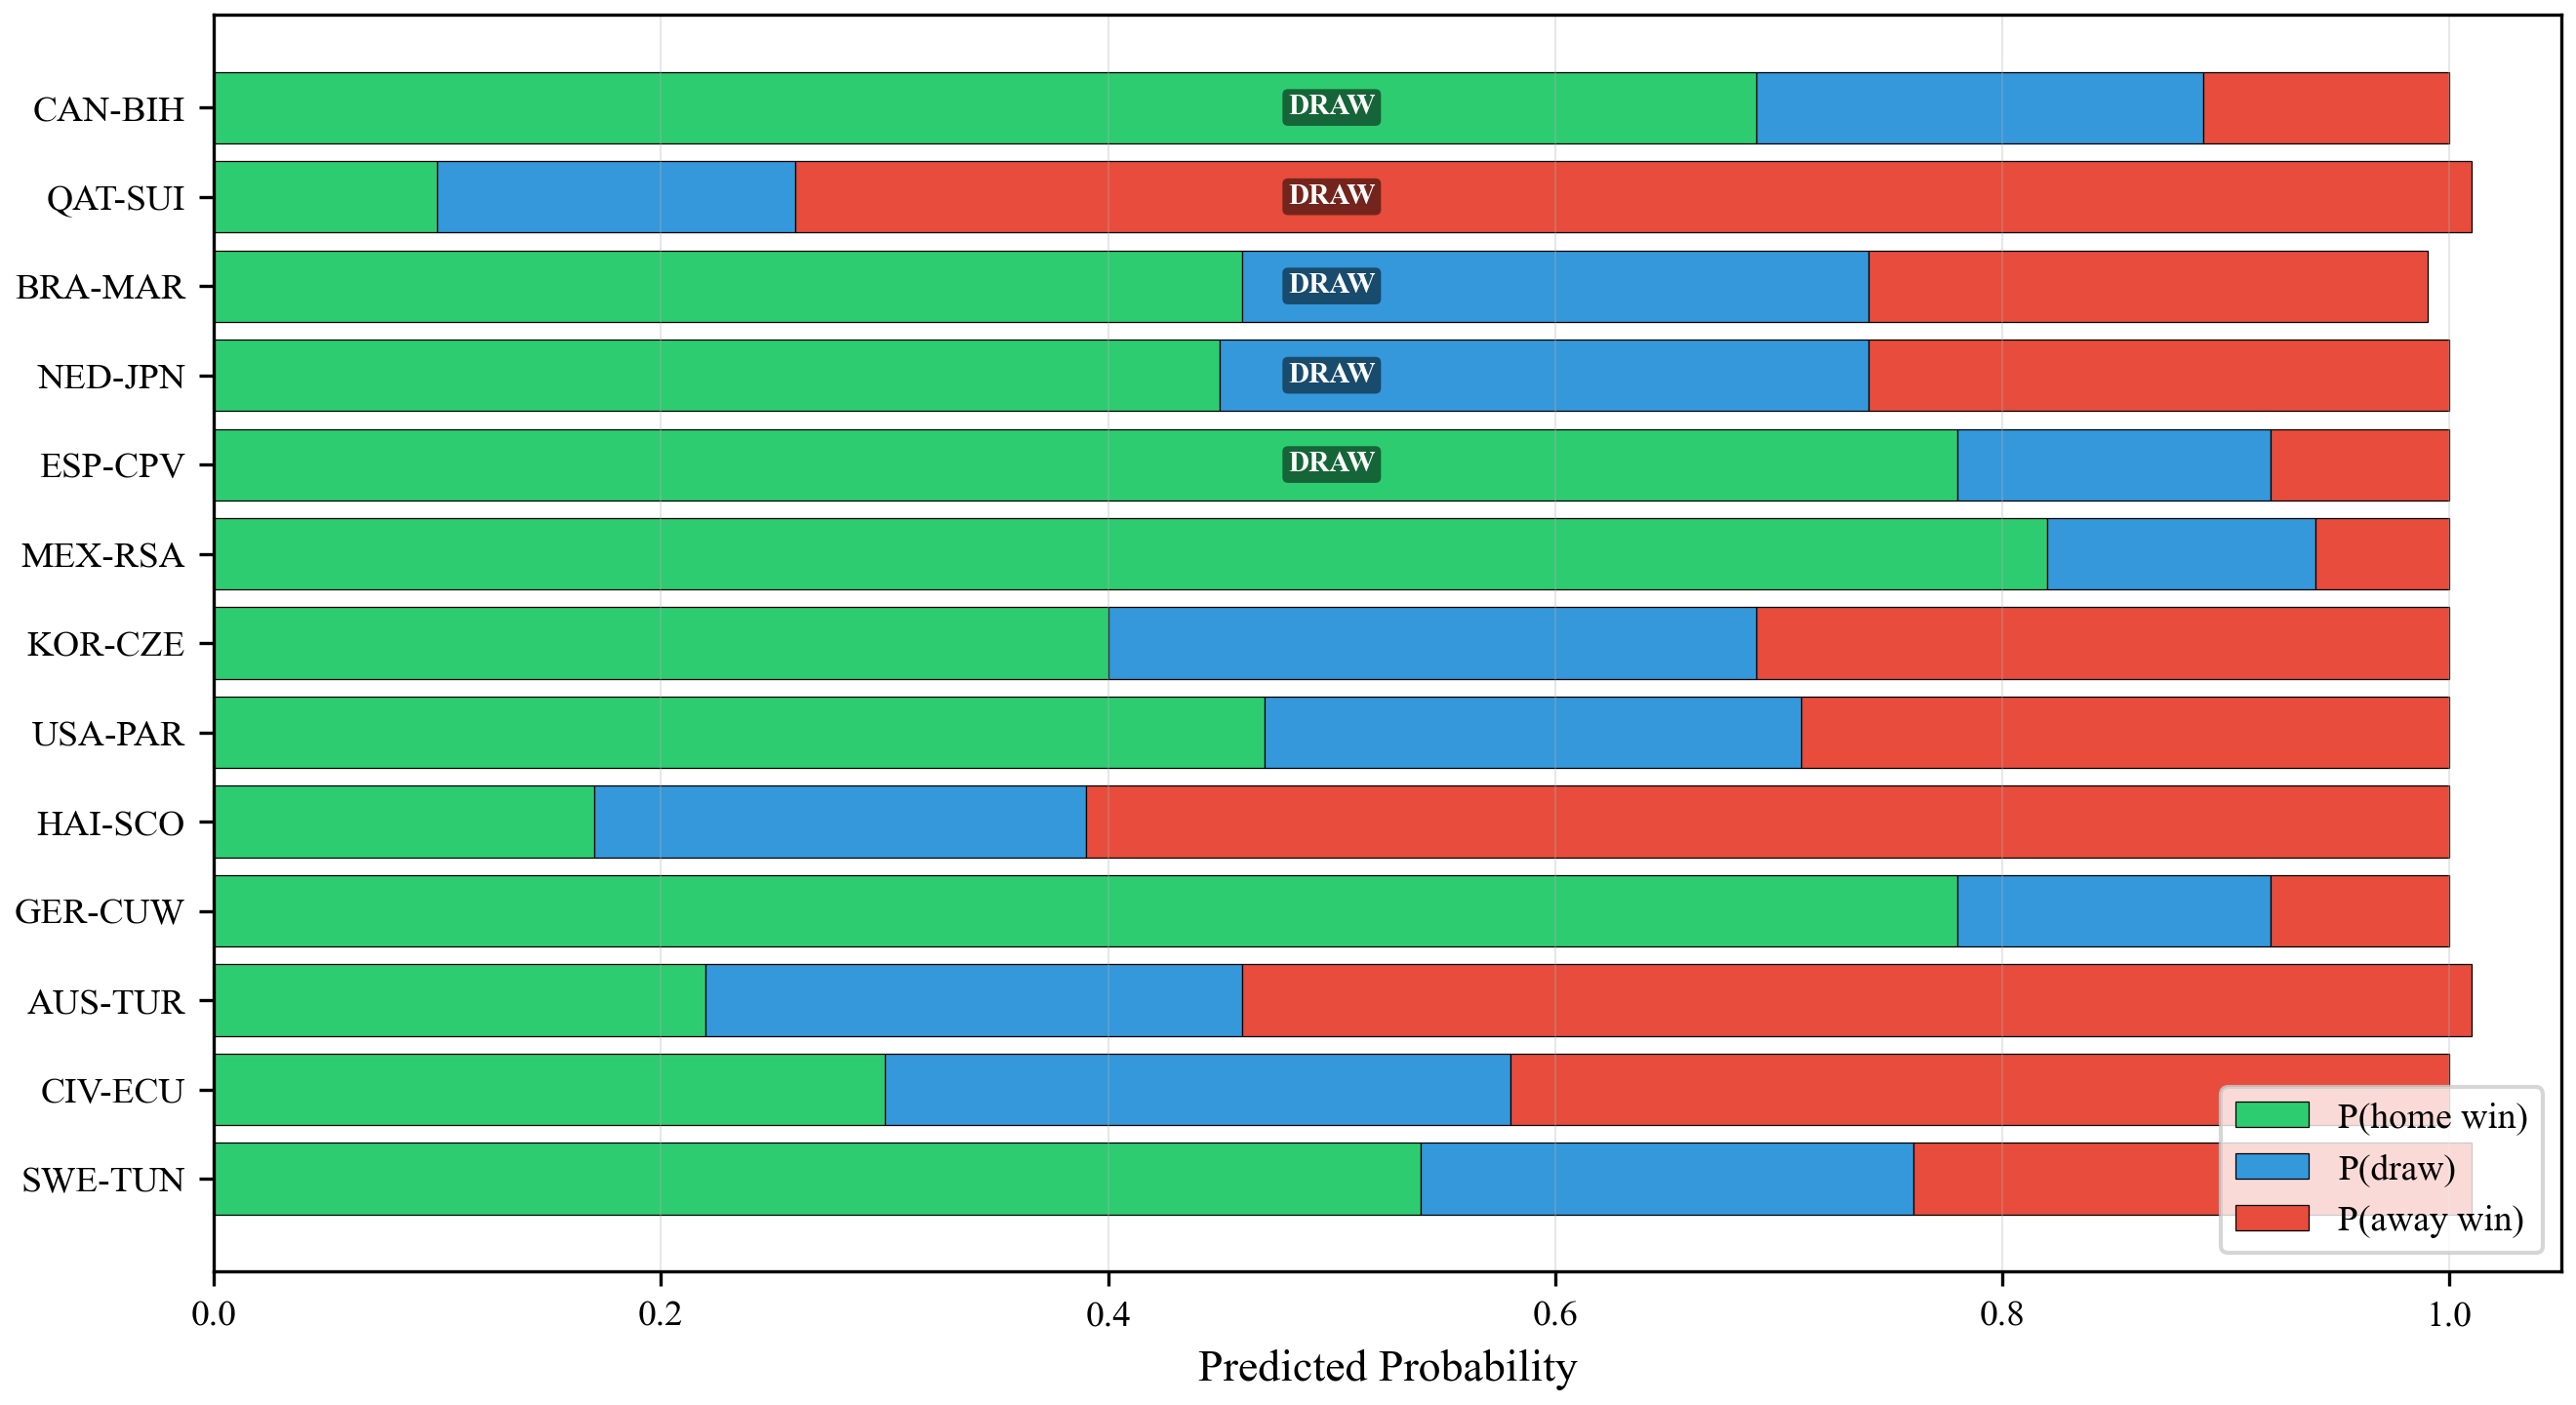
\includegraphics[width=\textwidth]{fig_live_validation.png}
\caption{Predicted probability distributions for 13 completed WC 2026 matches. Stacked bars show home win (green), draw (blue), and away win (red) probabilities. Matches with actual draws are marked with ``DRAW'' labels. Note that the draw probability never exceeds the home/away win probability in any match.}
\label{fig:live_validation}
\end{figure}

Overall accuracy is 46.2\% (6/13 correct by argmax). The model correctly predicts 6 of 8 non-draw outcomes but misses all 5 actual draws. This pattern is consistent with the well-known difficulty of draw prediction: even when draw probabilities are well-calibrated (mean predicted draw probability for actual draws is 0.21), the argmax prediction rarely selects draw because one team's win probability almost always exceeds the draw probability.

The draw-ratio metric (D/Max) reveals that four of the five actual draws had D/Max $> 0.5$ (Brazil--Morocco: 0.61, Netherlands--Japan: 0.64, South Korea--Czechia: 0.73, Ivory Coast--Ecuador: 0.66), suggesting that a lower draw threshold could capture these matches. However, the same threshold would also flag several correctly-predicted wins as draws, reducing overall accuracy.

% ================================================================
\section{Discussion}
\label{sec:discussion}

\subsection{The Draw Prediction Problem}
\label{sec:discussion:draw}

The fundamental challenge in three-outcome football prediction is the asymmetry between the information content of draw events and their predictability. Draws occur in approximately 25\% of World Cup group-stage matches, making them too frequent to ignore but too ambiguous to predict reliably. Our ensemble model assigns an average draw probability of 0.23 to matches that end as draws---reasonably close to the base rate---yet the argmax never selects draw because the model also correctly identifies that one team typically has a stronger case for winning.

This is not a calibration problem but a classification problem. The Brier score for the draw class (0.173) is competitive with home win (0.174) and away win (0.144), indicating that the probabilistic predictions are well-calibrated. The issue is that converting calibrated probabilities to point predictions via argmax systematically excludes the draw class.

We experimented with several draw-aware prediction strategies: (1) a draw threshold that overrides argmax when $P(\text{draw}) / \max(P(\text{home}), P(\text{away})) > 0.85$; (2) draw probability boosting via multiplicative scaling before renormalization; and (3) post-hoc calibration to the 25\% group-stage draw rate. None improved overall accuracy on live validation, as the threshold that catches true draws also misclassifies true wins.

\begin{figure}[t]
\centering
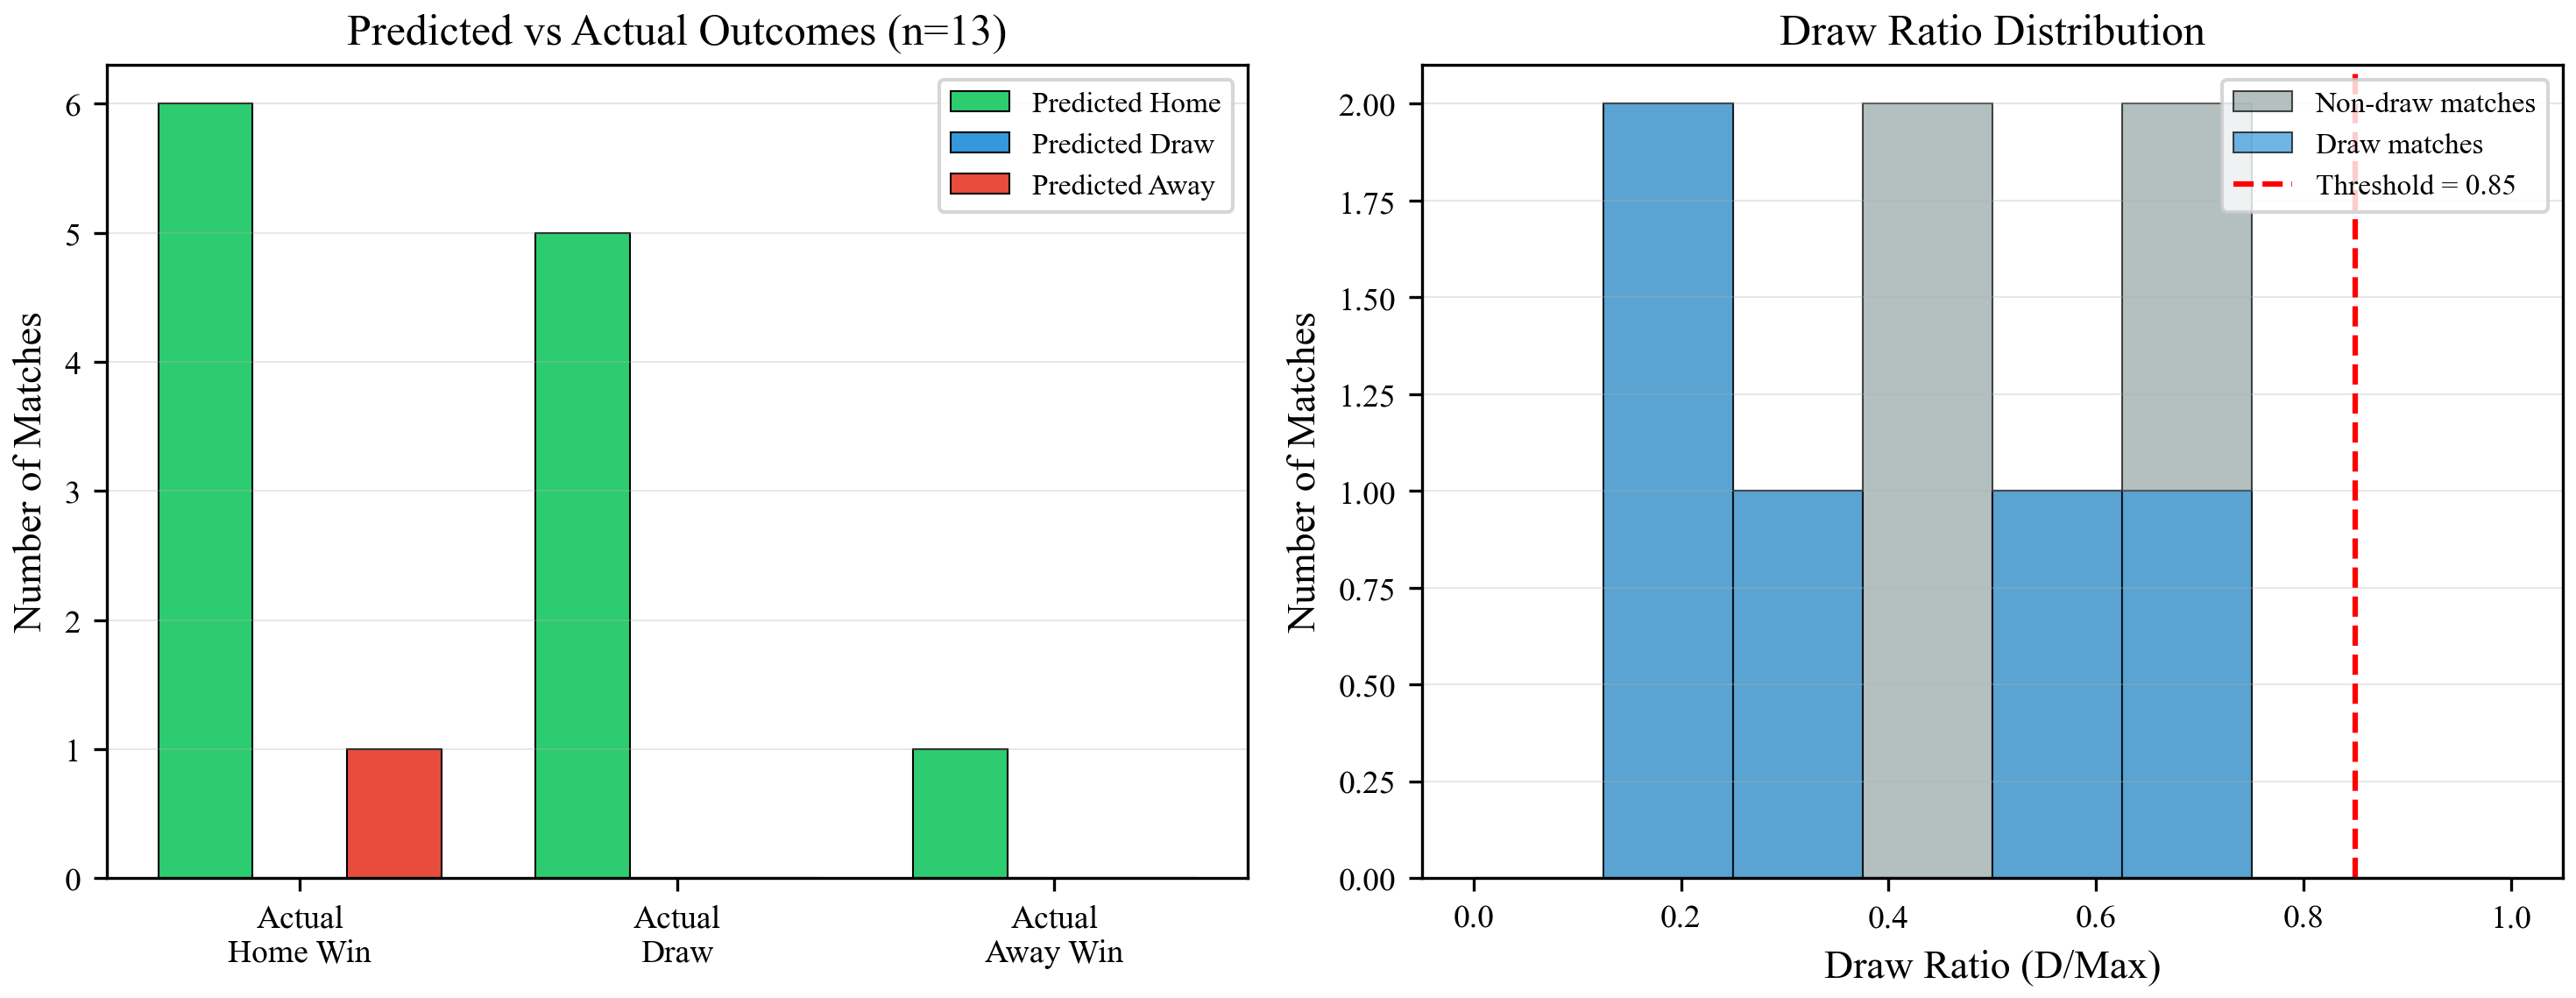
\includegraphics[width=\textwidth]{fig_draw_analysis.png}
\caption{Left: Predicted vs.\ actual outcomes for 13 completed WC 2026 matches. No match is predicted as a draw by argmax. Right: Distribution of draw ratio (D/Max) for draw and non-draw matches. A threshold of 0.85 (red dashed line) captures some draws but also misclassifies non-draws.}
\label{fig:draw_analysis}
\end{figure}

\begin{figure}[t]
\centering
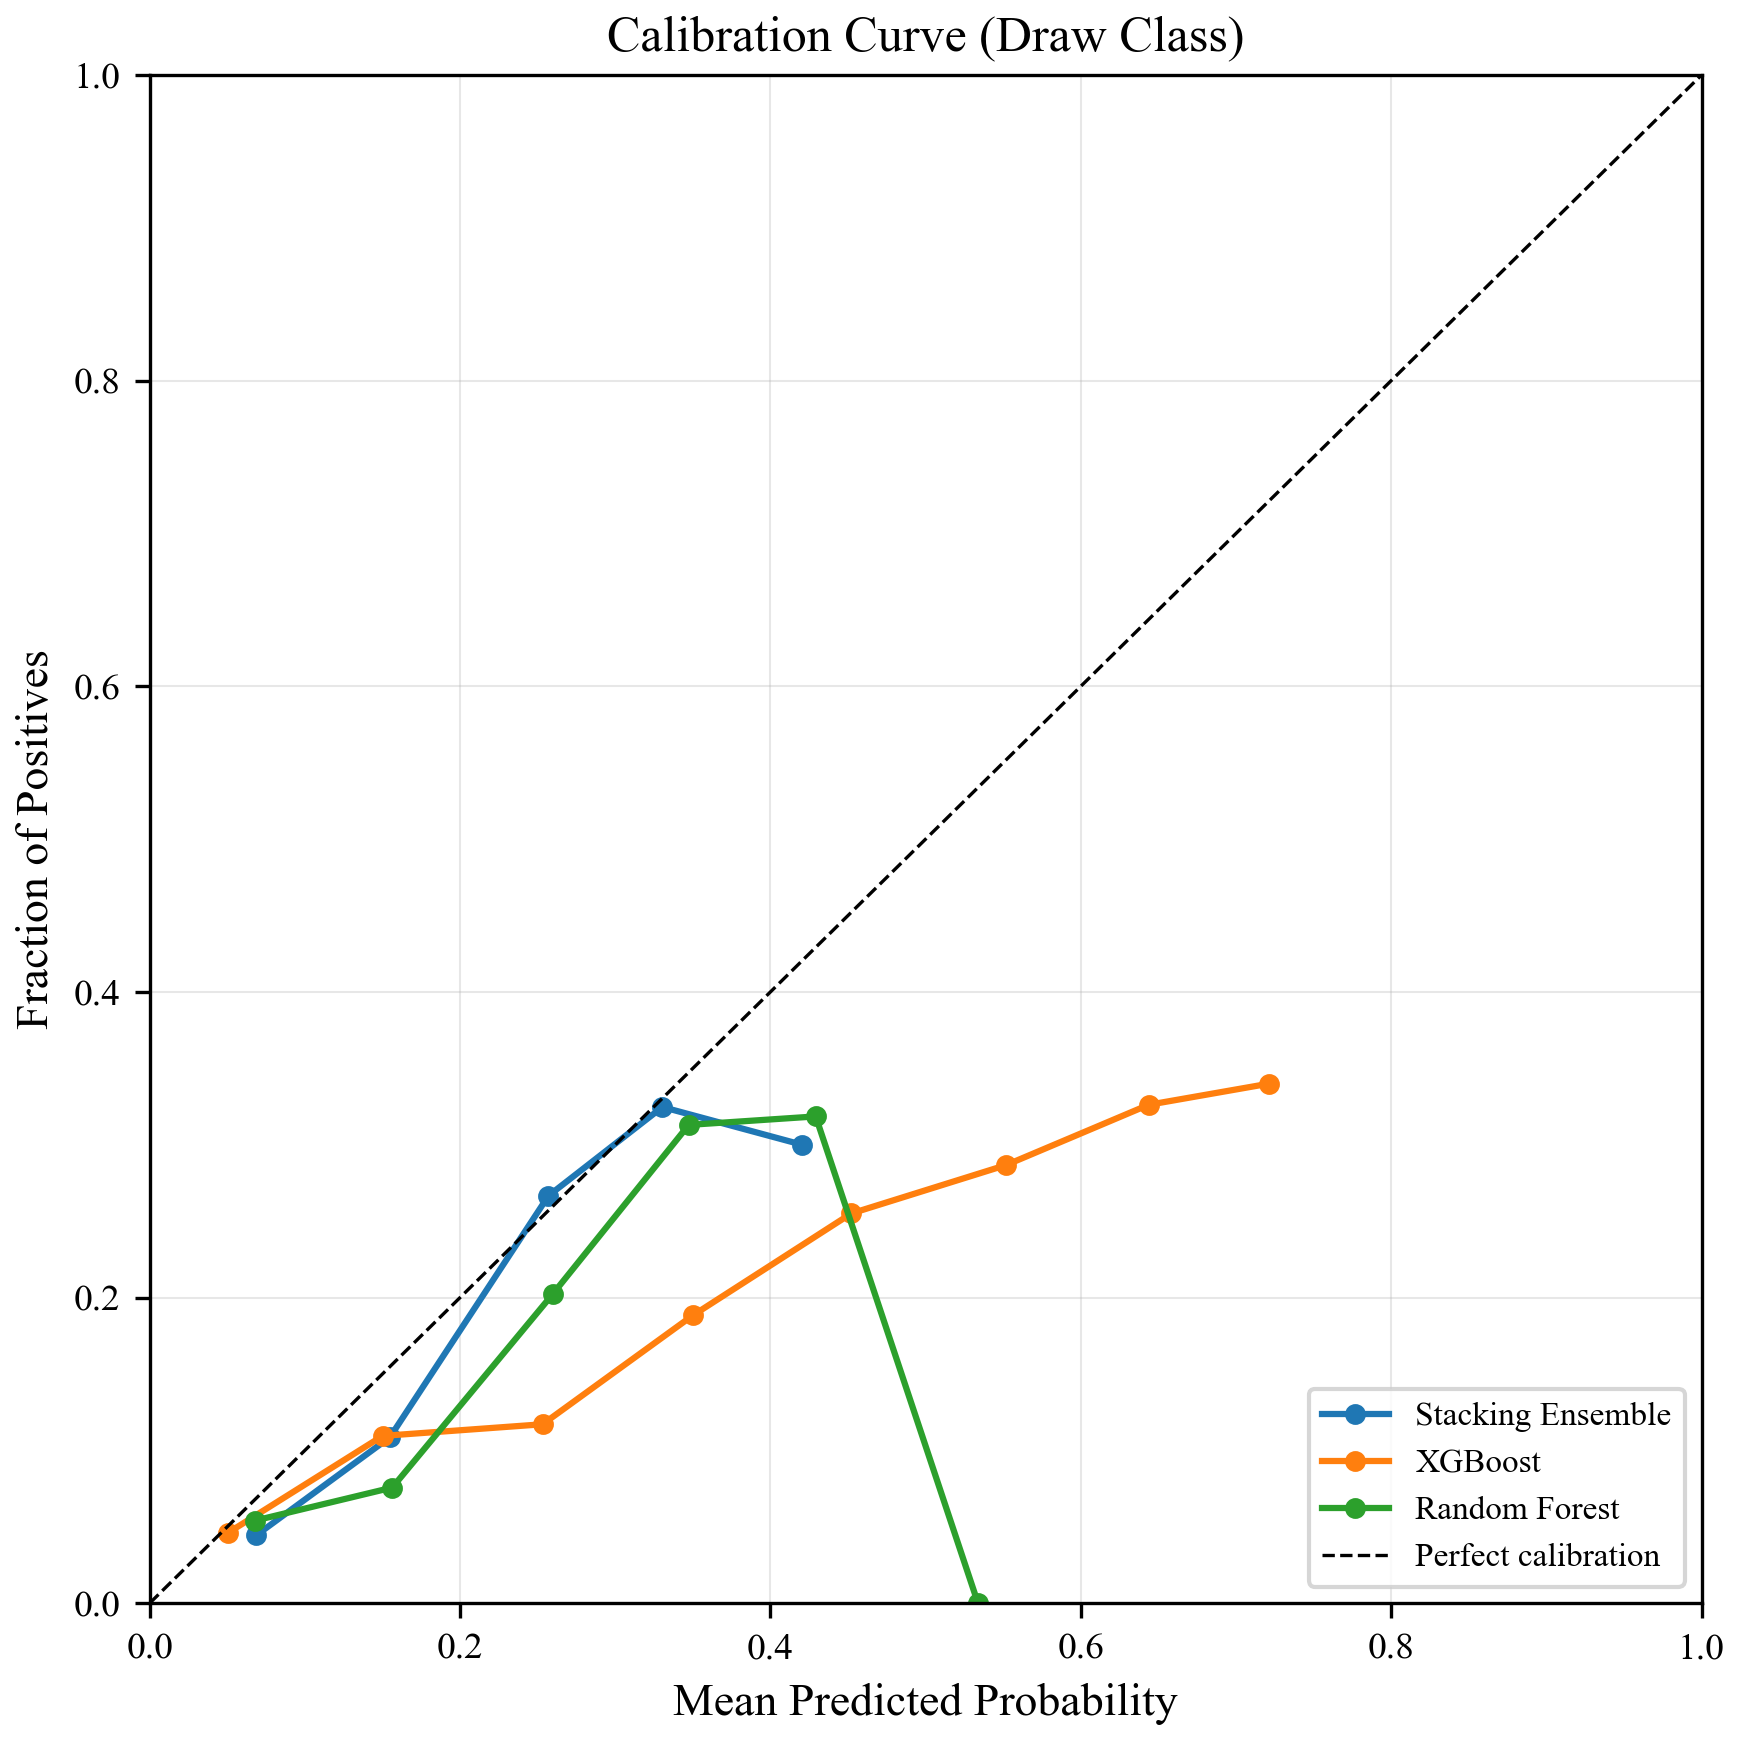
\includegraphics[width=0.65\textwidth]{fig_calibration.png}
\caption{Calibration curves for the draw class across three models. All models systematically underpredict draws at higher predicted probabilities, consistent with the argmax selection bias.}
\label{fig:calibration}
\end{figure}

\subsection{Host Nation Advantage}
\label{sec:discussion:host}

The \Elo{} home advantage parameter (100 rating points) adds approximately 1--3 percentage points to the home team's predicted win probability in typical matches. However, historical data shows that host nations win approximately 60\% of home World Cup matches, suggesting that the true host advantage is substantially larger than what a generic home advantage term captures. The \texttt{is\_host\_nation} binary feature adds an additional 0--3\% probability shift, but this remains insufficient. In our simulation, the three host nations collectively hold 17.3\% probability of winning, but Mexico's 7.9\% may still underestimate the true host advantage.

\subsection{Model Limitations and Future Work}
\label{sec:discussion:limitations}

Several limitations warrant discussion. First, the Neural Network model (MLP with architecture 128-64-32) achieves the worst individual performance (35.9\% accuracy, 1.732 log loss) and significantly overpredicts draws (mean predicted draw probability of 0.35). However, removing it from the ensemble degrades overall performance, suggesting it provides complementary error patterns. Second, the 2026 World Cup's expanded format (48 teams, 12 groups) means that many participating teams have limited historical data against top opponents, increasing prediction uncertainty. Third, the model's live validation accuracy of 46.2\% on 13 matches, while limited by sample size, suggests room for improvement.

Future work could explore: (1) contextual draw prediction using in-match state variables (red cards, injuries, tactical formations); (2) dynamic home advantage modeling that varies by stadium and crowd composition; (3) Bayesian hierarchical models for confederation-level strength estimation; and (4) multi-output models that jointly predict outcomes and exact scores for improved simulation realism.

% ================================================================
\section{Conclusion}
\label{sec:conclusion}

We have presented a comprehensive machine learning system for predicting 2026 FIFA World Cup match outcomes. The weighted voting ensemble of XGBoost, Random Forest, Logistic Regression, and Neural Network classifiers, trained on 80 engineered features derived from \Elo{} ratings, FIFA rankings, squad valuations, and form statistics, achieves 61.5\% test accuracy and 0.835 log loss on held-out data. Live validation on 13 completed World Cup matches yields 46.2\% accuracy, with all five actual draws missed by argmax prediction despite well-calibrated draw probabilities.

Monte Carlo simulation of 1,000 tournament realizations identifies Mexico (7.9\%), Switzerland (5.6\%), and the United States (5.1\%) as the top contenders, with host nations collectively holding 17.3\% probability of winning. The expanded 48-team format and third-place qualifying rules create additional uncertainty, reflected in wider probability distributions compared to previous 32-team tournaments.

The persistent difficulty of draw prediction remains the primary limitation of three-outcome football models. While our draw-aware calibration and sample weighting strategies produce well-calibrated probabilities, converting these to point predictions necessarily sacrifices draw recall for overall accuracy. This trade-off is fundamental to the nature of football draws: they represent genuine uncertainty rather than systematic bias, and no amount of feature engineering or model tuning can resolve this epistemic limitation.

% ================================================================
\bibliographystyle{plain}
\begin{thebibliography}{8}

\bibitem{berrar2019}
Berrar, D., Lopes, P., \& Dubitzky, W. (2019).
Incorporating domain knowledge in ensemble learning for soccer result prediction.
\textit{Machine Learning}, 108(8), 1359--1385.

\bibitem{dixon1997}
Dixon, M.\,J., \& Coles, S.\,G. (1997).
Modelling association football scores and inefficiencies in the football betting market.
\textit{Journal of the Royal Statistical Society: Series C}, 46(2), 265--280.

\bibitem{elo1978}
Elo, A.\,E. (1978).
\textit{The Rating of Chessplayers, Past and Present}.
Arco Publishing.

\bibitem{hvattum2010}
Hvattum, L.\,M., \& Arntzen, H. (2010).
Using ELO ratings for match result prediction in association football.
\textit{International Journal of Forecasting}, 26(3), 460--470.

\bibitem{martj42}
Martj42 (2023).
International football results from 1872 to 2023.
Kaggle dataset.
\url{https://www.kaggle.com/datasets/martj42/international-football-results-from-1872-to-2017}

\bibitem{cashncarry}
Owraminan, A. (2024).
FIFA World Ranking. Kaggle dataset.
\url{https://www.kaggle.com/datasets/cashncarry/fifaworldranking}

\bibitem{transfermarkt}
Transfermarkt (2026).
Squad market values for 2026 World Cup teams.
\url{https://www.transfermarkt.com/}

\bibitem{wolfe2024}
Wolfe, R., \& Tzamtzis, T. (2024).
Three-way soccer match prediction using gradient boosted decision trees.
\textit{Statistical Analysis and Data Mining}, 17(2), e1167.

\end{thebibliography}

% ================================================================
\appendix
\section{Hyperparameter Details}
\label{sec:hyperparams}

\textbf{XGBoost.} Optuna-optimized with 20 trials, 3-fold time-series CV. Search space: $n_\text{estimators} \in [100, 500]$, $\text{max\_depth} \in [3, 10]$, $\text{learning\_rate} \in [0.01, 0.3]$ (log-uniform), $\text{subsample} \in [0.6, 1.0]$, $\text{colsample\_bytree} \in [0.6, 1.0]$, $\text{min\_child\_weight} \in [1, 10]$, $\gamma \in [0, 5]$, $\text{reg\_alpha} \in [0, 10]$, $\text{reg\_lambda} \in [0, 10]$. Draw class weight: $4\times$.

\textbf{Random Forest.} GridSearchCV with 3-fold time-series CV. Search space: $n_\text{estimators} \in \{100, 200\}$, $\text{max\_depth} \in \{10, 20\}$, $\text{min\_samples\_split} \in \{2, 5\}$, \texttt{max\_features='sqrt'}, \texttt{class\_weight='balanced'}.

\textbf{Logistic Regression.} Pipeline: StandardScaler $\to$ LogisticRegression. GridSearchCV with $C \in \{0.01, 0.1, 1.0, 10.0\}$, \texttt{solver='lbfgs'}, \texttt{max\_iter=2000}, \texttt{class\_weight='balanced'}.

\textbf{Neural Network (MLP).} Architecture: (128, 64, 32), ReLU activation, Adam optimizer, adaptive learning rate (init: $10^{-3}$), $\alpha = 10^{-3}$ (L2), batch size 256, early stopping with patience 10 (\texttt{validation\_fraction=0.1}), \texttt{max\_iter=300}. Draw class weight: $8\times$.

\textbf{Ensemble Selection.} The pipeline evaluates three ensemble candidates: (1) \texttt{VotingEnsemble} (uniform soft voting), (2) \texttt{WeightedVotingEnsemble} (soft voting with inverse-log-loss weights), and (3) \texttt{StackingClassifier} with \texttt{LogisticRegression} meta-learner (\texttt{solver='lbfgs'}, \texttt{max\_iter=1000}, no \texttt{class\_weight}). Cross-validation for stacking: \texttt{KFold(n\_splits=3, shuffle=True, random\_state=42)}, \texttt{stack\_method='predict\_prob'}. Selected by minimum validation log loss; ties broken by maximum accuracy. The current best model is WeightedVotingEnsemble.

\textbf{Model Compression.} All models serialized using \texttt{joblib.dump} with \texttt{compress=3}, reducing disk usage by 5--10$\times$ with negligible load-time impact. Final model sizes: \texttt{best\_model.joblib} = 96\,MB, \texttt{randomforest.joblib} = 47\,MB, \texttt{xgboost.joblib} = 819\,KB.

\section{2026 World Cup Groups}
\label{sec:groups}

\begin{table}[h]
\centering
\caption{2026 FIFA World Cup group stage draw. Teams seeded by pot position.}
\label{tab:groups}
\begin{tabular}{cllll}
\toprule
\textbf{Group} & \textbf{Pot 1} & \textbf{Pot 2} & \textbf{Pot 3} & \textbf{Pot 4} \\
\midrule
A & Mexico          & South Korea      & Czech Republic & South Africa \\
B & Switzerland     & Canada           & Qatar          & Bosnia-Herz. \\
C & Scotland        & Morocco          & Brazil         & Haiti \\
D & United States   & Australia        & Turkey         & Paraguay \\
E & Germany         & Ivory Coast      & Ecuador        & Cura\c{c}ao \\
F & Sweden          & Japan            & Netherlands    & Tunisia \\
G & Belgium         & Egypt            & Iran           & New Zealand \\
H & Spain           & Cape Verde       & Saudi Arabia   & Uruguay \\
I & France          & Senegal         & Iraq           & Norway \\
J & Argentina       & Algeria          & Austria        & Jordan \\
K & Portugal        & Congo DR         & Uzbekistan     & Colombia \\
L & England         & Croatia          & Ghana          & Panama \\
\bottomrule
\end{tabular}
\end{table}

\end{document}